\documentclass[]{article}
\usepackage{lmodern}
\usepackage{amssymb,amsmath}
\usepackage{ifxetex,ifluatex}
\usepackage{fixltx2e} % provides \textsubscript
\ifnum 0\ifxetex 1\fi\ifluatex 1\fi=0 % if pdftex
  \usepackage[T1]{fontenc}
  \usepackage[utf8]{inputenc}
\else % if luatex or xelatex
  \ifxetex
    \usepackage{mathspec}
  \else
    \usepackage{fontspec}
  \fi
  \defaultfontfeatures{Ligatures=TeX,Scale=MatchLowercase}
\fi
% use upquote if available, for straight quotes in verbatim environments
\IfFileExists{upquote.sty}{\usepackage{upquote}}{}
% use microtype if available
\IfFileExists{microtype.sty}{%
\usepackage{microtype}
\UseMicrotypeSet[protrusion]{basicmath} % disable protrusion for tt fonts
}{}
\usepackage[margin=1in]{geometry}
\usepackage{hyperref}
\hypersetup{unicode=true,
            pdftitle={Course Project 2},
            pdfauthor={Devin Romines and Joseph Audras},
            pdfborder={0 0 0},
            breaklinks=true}
\urlstyle{same}  % don't use monospace font for urls
\usepackage{color}
\usepackage{fancyvrb}
\newcommand{\VerbBar}{|}
\newcommand{\VERB}{\Verb[commandchars=\\\{\}]}
\DefineVerbatimEnvironment{Highlighting}{Verbatim}{commandchars=\\\{\}}
% Add ',fontsize=\small' for more characters per line
\usepackage{framed}
\definecolor{shadecolor}{RGB}{248,248,248}
\newenvironment{Shaded}{\begin{snugshade}}{\end{snugshade}}
\newcommand{\KeywordTok}[1]{\textcolor[rgb]{0.13,0.29,0.53}{\textbf{{#1}}}}
\newcommand{\DataTypeTok}[1]{\textcolor[rgb]{0.13,0.29,0.53}{{#1}}}
\newcommand{\DecValTok}[1]{\textcolor[rgb]{0.00,0.00,0.81}{{#1}}}
\newcommand{\BaseNTok}[1]{\textcolor[rgb]{0.00,0.00,0.81}{{#1}}}
\newcommand{\FloatTok}[1]{\textcolor[rgb]{0.00,0.00,0.81}{{#1}}}
\newcommand{\ConstantTok}[1]{\textcolor[rgb]{0.00,0.00,0.00}{{#1}}}
\newcommand{\CharTok}[1]{\textcolor[rgb]{0.31,0.60,0.02}{{#1}}}
\newcommand{\SpecialCharTok}[1]{\textcolor[rgb]{0.00,0.00,0.00}{{#1}}}
\newcommand{\StringTok}[1]{\textcolor[rgb]{0.31,0.60,0.02}{{#1}}}
\newcommand{\VerbatimStringTok}[1]{\textcolor[rgb]{0.31,0.60,0.02}{{#1}}}
\newcommand{\SpecialStringTok}[1]{\textcolor[rgb]{0.31,0.60,0.02}{{#1}}}
\newcommand{\ImportTok}[1]{{#1}}
\newcommand{\CommentTok}[1]{\textcolor[rgb]{0.56,0.35,0.01}{\textit{{#1}}}}
\newcommand{\DocumentationTok}[1]{\textcolor[rgb]{0.56,0.35,0.01}{\textbf{\textit{{#1}}}}}
\newcommand{\AnnotationTok}[1]{\textcolor[rgb]{0.56,0.35,0.01}{\textbf{\textit{{#1}}}}}
\newcommand{\CommentVarTok}[1]{\textcolor[rgb]{0.56,0.35,0.01}{\textbf{\textit{{#1}}}}}
\newcommand{\OtherTok}[1]{\textcolor[rgb]{0.56,0.35,0.01}{{#1}}}
\newcommand{\FunctionTok}[1]{\textcolor[rgb]{0.00,0.00,0.00}{{#1}}}
\newcommand{\VariableTok}[1]{\textcolor[rgb]{0.00,0.00,0.00}{{#1}}}
\newcommand{\ControlFlowTok}[1]{\textcolor[rgb]{0.13,0.29,0.53}{\textbf{{#1}}}}
\newcommand{\OperatorTok}[1]{\textcolor[rgb]{0.81,0.36,0.00}{\textbf{{#1}}}}
\newcommand{\BuiltInTok}[1]{{#1}}
\newcommand{\ExtensionTok}[1]{{#1}}
\newcommand{\PreprocessorTok}[1]{\textcolor[rgb]{0.56,0.35,0.01}{\textit{{#1}}}}
\newcommand{\AttributeTok}[1]{\textcolor[rgb]{0.77,0.63,0.00}{{#1}}}
\newcommand{\RegionMarkerTok}[1]{{#1}}
\newcommand{\InformationTok}[1]{\textcolor[rgb]{0.56,0.35,0.01}{\textbf{\textit{{#1}}}}}
\newcommand{\WarningTok}[1]{\textcolor[rgb]{0.56,0.35,0.01}{\textbf{\textit{{#1}}}}}
\newcommand{\AlertTok}[1]{\textcolor[rgb]{0.94,0.16,0.16}{{#1}}}
\newcommand{\ErrorTok}[1]{\textcolor[rgb]{0.64,0.00,0.00}{\textbf{{#1}}}}
\newcommand{\NormalTok}[1]{{#1}}
\usepackage{graphicx,grffile}
\makeatletter
\def\maxwidth{\ifdim\Gin@nat@width>\linewidth\linewidth\else\Gin@nat@width\fi}
\def\maxheight{\ifdim\Gin@nat@height>\textheight\textheight\else\Gin@nat@height\fi}
\makeatother
% Scale images if necessary, so that they will not overflow the page
% margins by default, and it is still possible to overwrite the defaults
% using explicit options in \includegraphics[width, height, ...]{}
\setkeys{Gin}{width=\maxwidth,height=\maxheight,keepaspectratio}
\IfFileExists{parskip.sty}{%
\usepackage{parskip}
}{% else
\setlength{\parindent}{0pt}
\setlength{\parskip}{6pt plus 2pt minus 1pt}
}
\setlength{\emergencystretch}{3em}  % prevent overfull lines
\providecommand{\tightlist}{%
  \setlength{\itemsep}{0pt}\setlength{\parskip}{0pt}}
\setcounter{secnumdepth}{0}
% Redefines (sub)paragraphs to behave more like sections
\ifx\paragraph\undefined\else
\let\oldparagraph\paragraph
\renewcommand{\paragraph}[1]{\oldparagraph{#1}\mbox{}}
\fi
\ifx\subparagraph\undefined\else
\let\oldsubparagraph\subparagraph
\renewcommand{\subparagraph}[1]{\oldsubparagraph{#1}\mbox{}}
\fi

%%% Use protect on footnotes to avoid problems with footnotes in titles
\let\rmarkdownfootnote\footnote%
\def\footnote{\protect\rmarkdownfootnote}

%%% Change title format to be more compact
\usepackage{titling}

% Create subtitle command for use in maketitle
\providecommand{\subtitle}[1]{
  \posttitle{
    \begin{center}\large#1\end{center}
    }
}

\setlength{\droptitle}{-2em}

  \title{Course Project 2}
    \pretitle{\vspace{\droptitle}\centering\huge}
  \posttitle{\par}
    \author{Devin Romines and Joseph Audras}
    \preauthor{\centering\large\emph}
  \postauthor{\par}
      \predate{\centering\large\emph}
  \postdate{\par}
    \date{May 13, 2019}


\begin{document}
\maketitle

\section{Introduction}\label{introduction}

Dataset Source:
\url{https://www.kaggle.com/lava18/google-play-store-apps}

\subsection{Description}\label{description}

The Google Play Store Data Set is a data set containing data on over
10,000 apps in the Google Play Store for Android products. The data set
looks at things such as rating, number of installations, and genre to
produce a plethora of information on each app. For this project, we
would like to see if the rating of the app can be accurately predicted
by the variables provided in the data set.

The data set was gathered from
\url{https://www.kaggle.com/lava18/google-play-store-apps} which was
last updated 2 months ago, giving us Version 6, with which we are
working. The data was posted by Lavanya Gupta, a software engineer at
HSBC Software Development in India. More information on her can be found
here \url{https://www.kaggle.com/lava18}. The information in the data
set was scraped from the Google Play Store by Lavanya Gupta, in an
effort to provide similar information on its apps as is publically
available from the Apple App Store so that developers may be more
inclined to work in the Android market.

\begin{Shaded}
\begin{Highlighting}[]
\KeywordTok{library}\NormalTok{(tidyverse)}
\KeywordTok{library}\NormalTok{(lubridate)}
\KeywordTok{library}\NormalTok{(ggplot2)}
\end{Highlighting}
\end{Shaded}

\section{Data Dictionary}\label{data-dictionary}

\begin{itemize}
\item
  App -- Factor, 9660 levels -- The name of the app.
\item
  Category -- Factor, 34 levels -- The general type of app, such as
  Dating, Cooking, or Art and Design
\item
  Rating -- Numerical, range from 0-5 -- The rating of the app on a
  scale from 0-5.
\item
  Reviews -- Number, very wide range -- The number of reviews that the
  app received.
\item
  Size (Removed in Cleaning) -- Factor, 462 levels -- The size in
  megabytes of the app.
\item
  Installs -- Number, given as a factor of 10 -- The number of
  installations an app received.
\item
  Type (Removed in Cleaning) -- Factor, 4 levels -- Whether or not the
  app is free.
\item
  Price -- Number, mostly 0 but some go very high -- The Price of the
  app.
\item
  Content.Rating -- Factor, 4 levels -- The rating for the app,
  Everyone, Everyone 10+, Mature 17+, and Teen.
\item
  Genres -- Factor, 120 levels -- The genre of the app, Action, Action
  and Adventure, etc.
\item
  Last.Updated -- Factor, 1378 levels -- The date on which the app was
  last updated, given in multiple formats.
\item
  Current.Ver (Removed in Cleaning) -- Factor, 2834 levels -- The
  current version of the app, 0.0.0.2, 0.0.1, etc.
\item
  Android.Ver (Removed in Cleaning) -- Factor, 35 levels -- The version
  of Android phone required to use the app, given in the form, ``version
  and up''
\end{itemize}

\section{Data Cleaning}\label{data-cleaning}

Here we load the data set.

\begin{Shaded}
\begin{Highlighting}[]
\NormalTok{RawData <-}\StringTok{ }\KeywordTok{read.csv}\NormalTok{(}\StringTok{"googleplaystore.csv"}\NormalTok{)}
\end{Highlighting}
\end{Shaded}

This next code removes a problematic row that we found to have severe
errors when it was inputed.

\begin{Shaded}
\begin{Highlighting}[]
\NormalTok{GooglePlayStore <-}\StringTok{ }\NormalTok{RawData[-}\KeywordTok{c}\NormalTok{(}\DecValTok{10473}\NormalTok{), ]}
\end{Highlighting}
\end{Shaded}

Some of the values in the data set for the Rating value, which is the
one we are looking at, read as NaN, so we will remove all entries that
contain that value.

\begin{Shaded}
\begin{Highlighting}[]
\NormalTok{GooglePlayStore <-}\StringTok{ }\NormalTok{GooglePlayStore[-}\KeywordTok{grep}\NormalTok{(}\StringTok{"NaN"}\NormalTok{, GooglePlayStore$Rating), ]}
\end{Highlighting}
\end{Shaded}

The Reviews variable was initially given as a factor variable. Here we
change that to be a numeric as it should be.

\begin{Shaded}
\begin{Highlighting}[]
\NormalTok{GooglePlayStore$Reviews <-}\StringTok{ }\KeywordTok{as.numeric}\NormalTok{(}\KeywordTok{as.character}\NormalTok{(GooglePlayStore$Reviews))}
\end{Highlighting}
\end{Shaded}

The size variable was deemed unnecessary for our goals for this project
so here we remove it.

\begin{Shaded}
\begin{Highlighting}[]
\NormalTok{GooglePlayStore <-}\StringTok{ }\NormalTok{GooglePlayStore[, -}\DecValTok{5}\NormalTok{]}
\end{Highlighting}
\end{Shaded}

The Installs variable was initially given as a factor, with undesirable
formatting. Here we remove the characters in the entries we do not want
and then convert the Installs variable to a numeric as desired.

\begin{Shaded}
\begin{Highlighting}[]
\NormalTok{GooglePlayStore$Installs <-}\StringTok{ }\KeywordTok{gsub}\NormalTok{(}\StringTok{"}\CharTok{\textbackslash{}\textbackslash{}}\StringTok{D"}\NormalTok{, }\StringTok{""}\NormalTok{, GooglePlayStore$Installs)}
\NormalTok{GooglePlayStore$Installs <-}\StringTok{ }\KeywordTok{as.numeric}\NormalTok{(}\KeywordTok{as.character}\NormalTok{(GooglePlayStore$Installs))}
\end{Highlighting}
\end{Shaded}

The Type variable merely indicates whether or not the app is free, which
is also given by the better variable, Price, so here we remove it.

\begin{Shaded}
\begin{Highlighting}[]
\NormalTok{GooglePlayStore <-}\StringTok{ }\NormalTok{GooglePlayStore[, -}\DecValTok{6}\NormalTok{]}
\end{Highlighting}
\end{Shaded}

The Price variable is interesting, here we had to remove the dollar sign
as we wanted to convert it to a numeric variable; however, when removing
the dollar sign we also noticed that the code also removed the decimal
point. To recover it, we simply divided every price by 100. This solved
the problem.

\begin{Shaded}
\begin{Highlighting}[]
\NormalTok{GooglePlayStore$Price <-}\StringTok{ }\KeywordTok{gsub}\NormalTok{(}\StringTok{"[[:punct:]]"}\NormalTok{, }\StringTok{""}\NormalTok{, GooglePlayStore$Price)}
\NormalTok{GooglePlayStore$Price <-}\StringTok{ }\KeywordTok{as.numeric}\NormalTok{(GooglePlayStore$Price)}
\NormalTok{GooglePlayStore$Price <-}\StringTok{ }\NormalTok{GooglePlayStore$Price/}\DecValTok{100}
\end{Highlighting}
\end{Shaded}

We determined that the Current.Ver variable was irrelevant to our goals,
so here we remove it.

\begin{Shaded}
\begin{Highlighting}[]
\NormalTok{GooglePlayStore <-}\StringTok{ }\NormalTok{GooglePlayStore[, -}\DecValTok{10}\NormalTok{]}
\end{Highlighting}
\end{Shaded}

We also determined that the Android.Ver variable was irrelevant to our
goals, so here we remove that as well.

\begin{Shaded}
\begin{Highlighting}[]
\NormalTok{GooglePlayStore <-}\StringTok{ }\NormalTok{GooglePlayStore[, -}\DecValTok{10}\NormalTok{]}
\end{Highlighting}
\end{Shaded}

Here we write the cleaned data set to disk.

\begin{Shaded}
\begin{Highlighting}[]
\KeywordTok{write.csv}\NormalTok{(GooglePlayStore,}\StringTok{"Prepared_Google_Play_Store_App_Data.csv"}\NormalTok{,}\DataTypeTok{row.names=}\OtherTok{FALSE}\NormalTok{)}
\end{Highlighting}
\end{Shaded}

Because we intend on making a predictive model, here we split the data
into a testing and training data set.

\begin{Shaded}
\begin{Highlighting}[]
\KeywordTok{set.seed}\NormalTok{(}\DecValTok{42}\NormalTok{)}

\NormalTok{GooglePlayStoreTemp <-}\StringTok{ }\NormalTok{GooglePlayStore %>%}\StringTok{ }\KeywordTok{mutate}\NormalTok{(}\DataTypeTok{id=}\KeywordTok{row_number}\NormalTok{())}
\NormalTok{Train <-}\StringTok{ }\NormalTok{GooglePlayStoreTemp %>%}\StringTok{ }\KeywordTok{sample_frac}\NormalTok{(}\FloatTok{0.6}\NormalTok{)}
\NormalTok{Test <-}\StringTok{ }\NormalTok{GooglePlayStoreTemp %>%}\StringTok{ }\KeywordTok{anti_join}\NormalTok{(Train,}\DataTypeTok{by=}\StringTok{"id"}\NormalTok{)}
\NormalTok{Train$id <-}\StringTok{ }\OtherTok{NULL}
\NormalTok{Test$id <-}\StringTok{ }\OtherTok{NULL}
\KeywordTok{write.csv}\NormalTok{(Test,}\StringTok{"Test.csv"}\NormalTok{,}\DataTypeTok{row.names =} \OtherTok{FALSE}\NormalTok{)}
\KeywordTok{rm}\NormalTok{(Test,GooglePlayStoreTemp)}
\end{Highlighting}
\end{Shaded}

\section{Exploratory Data Analysis}\label{exploratory-data-analysis}

To begin the exploratory data analysis, let's look at the data set as a
whole.

\begin{Shaded}
\begin{Highlighting}[]
\KeywordTok{summary}\NormalTok{(Train)}
\end{Highlighting}
\end{Shaded}

\begin{verbatim}
##                                                  App      
##  Candy Crush Saga                                  :   6  
##  ROBLOX                                            :   6  
##  Bleacher Report: sports news, scores, & highlights:   5  
##  Duolingo: Learn Languages Free                    :   5  
##  ESPN                                              :   5  
##  8 Ball Pool                                       :   4  
##  (Other)                                           :5589  
##                Category        Rating         Reviews        
##  FAMILY            :1058   Min.   :1.000   Min.   :       1  
##  GAME              : 638   1st Qu.:4.000   1st Qu.:     174  
##  TOOLS             : 455   Median :4.300   Median :    5417  
##  MEDICAL           : 207   Mean   :4.183   Mean   :  503129  
##  SPORTS            : 205   3rd Qu.:4.500   3rd Qu.:   77868  
##  HEALTH_AND_FITNESS: 203   Max.   :5.000   Max.   :78158306  
##  (Other)           :2854                                     
##     Installs             Price                 Content.Rating
##  Min.   :1.000e+00   Min.   :  0.000                  :   0  
##  1st Qu.:1.000e+04   1st Qu.:  0.000   Adults only 18+:   3  
##  Median :5.000e+05   Median :  0.000   Everyone       :4434  
##  Mean   :1.716e+07   Mean   :  1.109   Everyone 10+   : 253  
##  3rd Qu.:5.000e+06   3rd Qu.:  0.000   Mature 17+     : 276  
##  Max.   :1.000e+09   Max.   :400.000   Teen           : 653  
##                                        Unrated        :   1  
##            Genres             Last.Updated 
##  Tools        : 455   August 1, 2018: 179  
##  Entertainment: 336   August 3, 2018: 178  
##  Education    : 281   July 31, 2018 : 164  
##  Action       : 213   August 2, 2018: 157  
##  Sports       : 211   July 30, 2018 : 114  
##  Medical      : 207   August 6, 2018:  99  
##  (Other)      :3917   (Other)       :4729
\end{verbatim}

\begin{Shaded}
\begin{Highlighting}[]
\KeywordTok{pairs}\NormalTok{(Train)}
\end{Highlighting}
\end{Shaded}

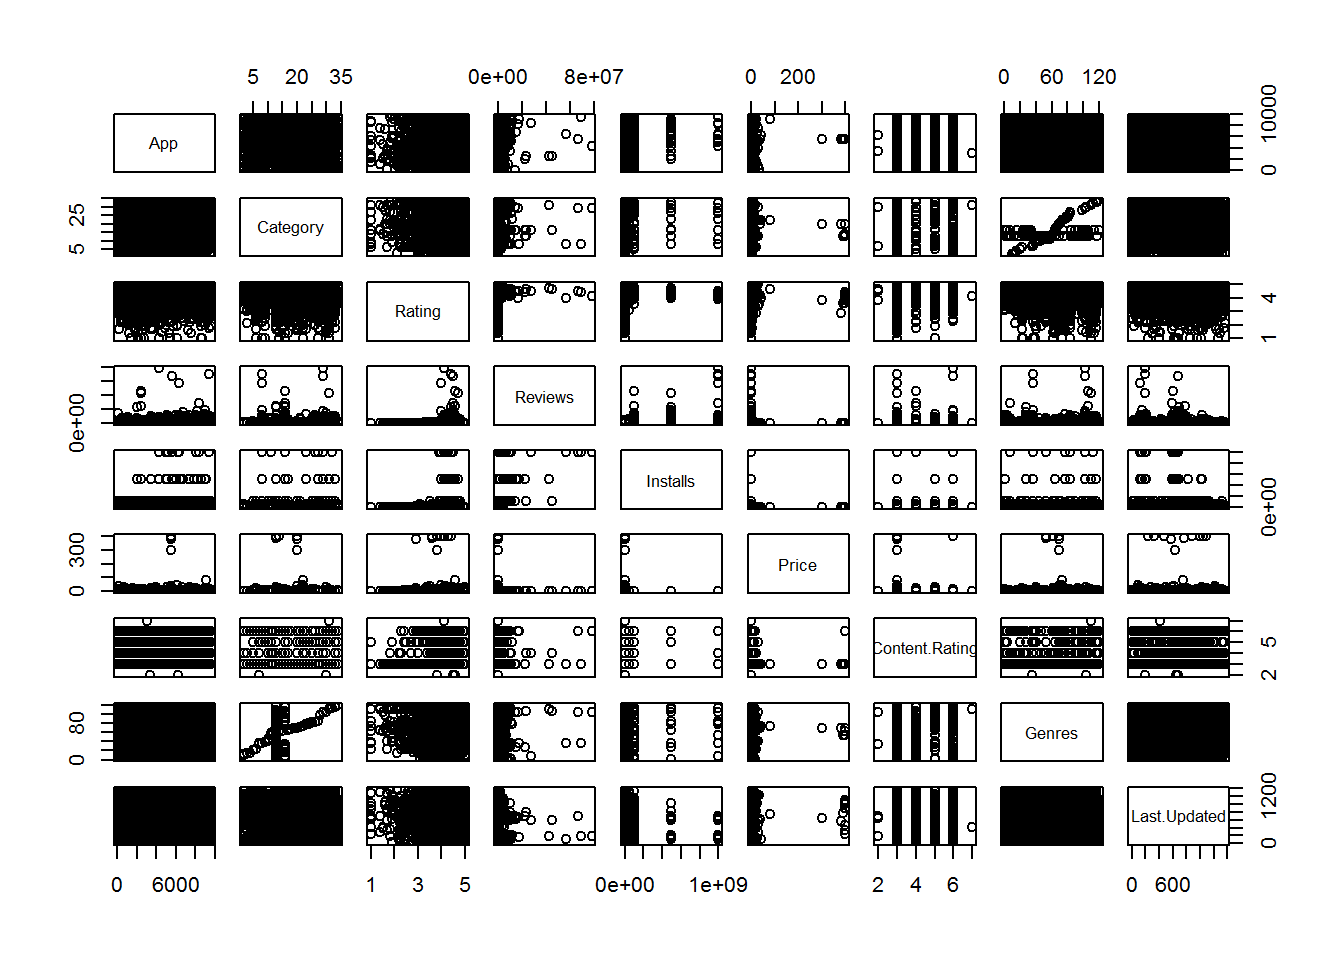
\includegraphics{Project_2_Work_files/figure-latex/unnamed-chunk-14-1.pdf}

Now, let's look at the individual variables.

\begin{Shaded}
\begin{Highlighting}[]
\KeywordTok{ggplot}\NormalTok{(Train) +}\StringTok{ }\KeywordTok{geom_bar}\NormalTok{(}\KeywordTok{aes}\NormalTok{(}\DataTypeTok{x=}\NormalTok{Category)) +}\StringTok{ }\KeywordTok{coord_flip}\NormalTok{()}
\end{Highlighting}
\end{Shaded}

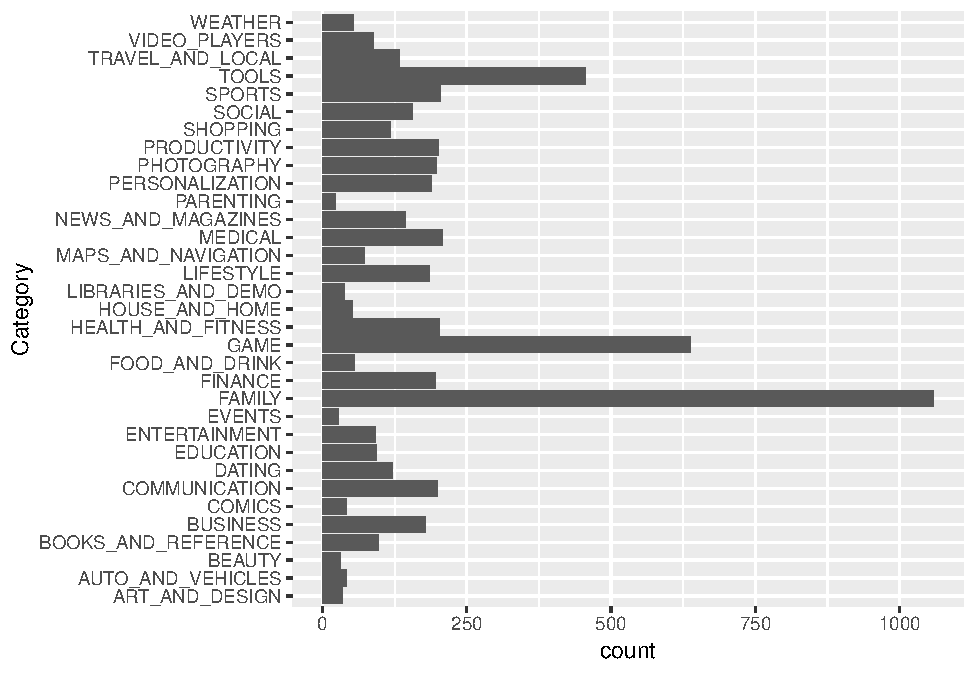
\includegraphics{Project_2_Work_files/figure-latex/unnamed-chunk-15-1.pdf}

\begin{Shaded}
\begin{Highlighting}[]
\KeywordTok{ggplot}\NormalTok{(Train) +}\StringTok{ }\KeywordTok{geom_density}\NormalTok{(}\KeywordTok{aes}\NormalTok{(}\DataTypeTok{x=}\NormalTok{Rating),}\DataTypeTok{fill=}\StringTok{"light blue"}\NormalTok{)}
\end{Highlighting}
\end{Shaded}

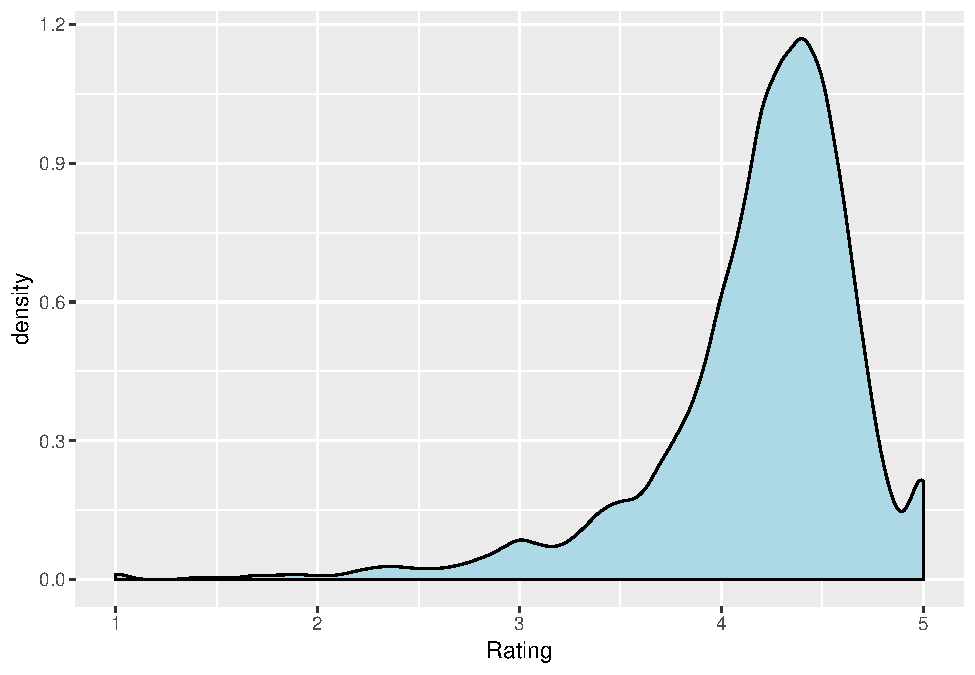
\includegraphics{Project_2_Work_files/figure-latex/unnamed-chunk-15-2.pdf}

\begin{Shaded}
\begin{Highlighting}[]
\KeywordTok{ggplot}\NormalTok{(Train) +}\StringTok{ }\KeywordTok{geom_density}\NormalTok{(}\KeywordTok{aes}\NormalTok{(}\DataTypeTok{x=}\KeywordTok{log}\NormalTok{(Reviews)),}\DataTypeTok{fill=}\StringTok{"light green"}\NormalTok{)}
\end{Highlighting}
\end{Shaded}

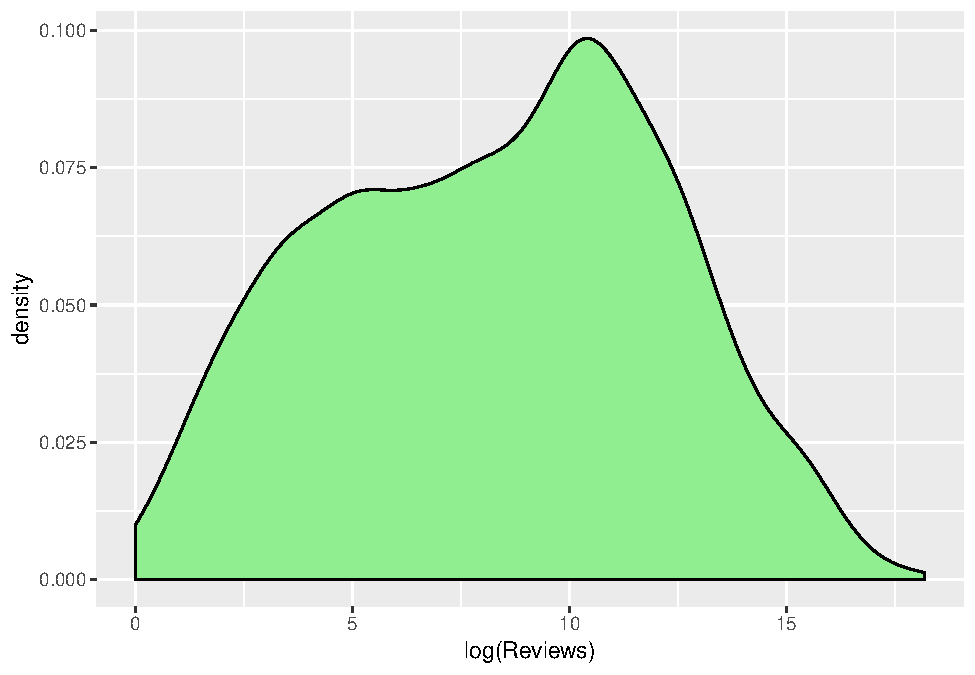
\includegraphics{Project_2_Work_files/figure-latex/unnamed-chunk-15-3.pdf}

\begin{Shaded}
\begin{Highlighting}[]
\KeywordTok{ggplot}\NormalTok{(Train) +}\StringTok{ }\KeywordTok{geom_bar}\NormalTok{(}\KeywordTok{aes}\NormalTok{(}\DataTypeTok{x=}\KeywordTok{log}\NormalTok{(Installs)),}\DataTypeTok{fill=}\StringTok{"purple"}\NormalTok{)}
\end{Highlighting}
\end{Shaded}

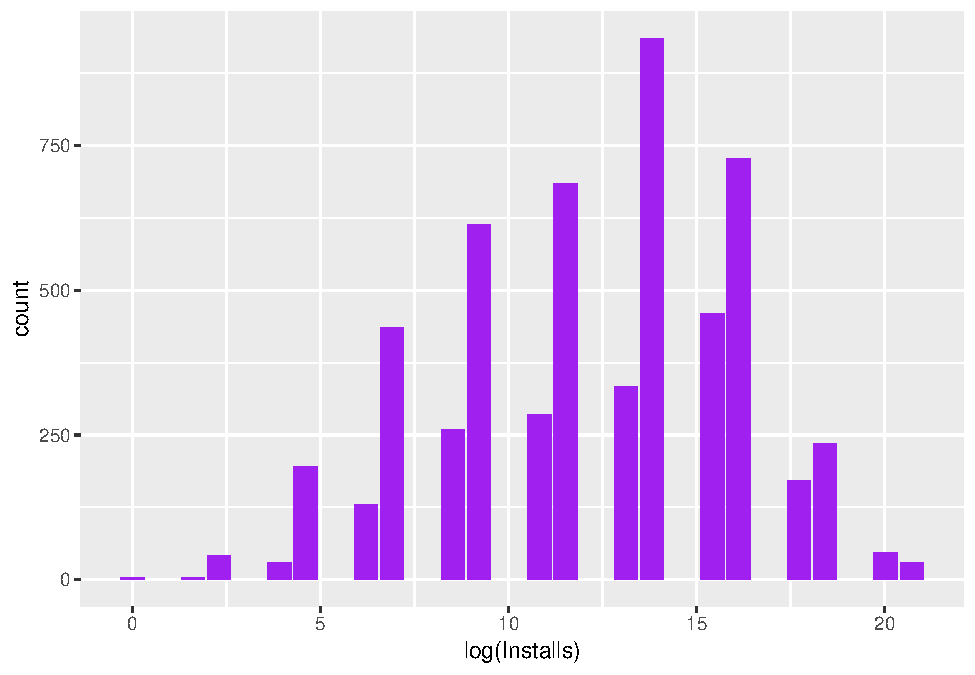
\includegraphics{Project_2_Work_files/figure-latex/unnamed-chunk-15-4.pdf}

\begin{Shaded}
\begin{Highlighting}[]
\KeywordTok{ggplot}\NormalTok{(Train) +}\StringTok{ }\KeywordTok{geom_density}\NormalTok{(}\KeywordTok{aes}\NormalTok{(}\DataTypeTok{x=}\KeywordTok{log}\NormalTok{(Price)),}\DataTypeTok{fill=}\StringTok{"gray"}\NormalTok{)}
\end{Highlighting}
\end{Shaded}

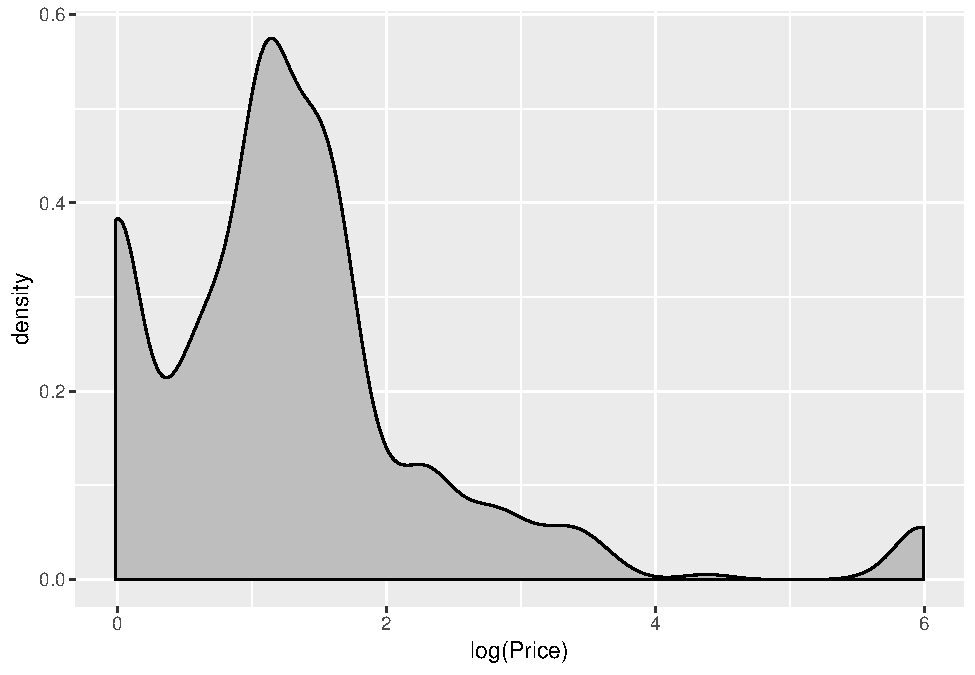
\includegraphics{Project_2_Work_files/figure-latex/unnamed-chunk-15-5.pdf}

\begin{Shaded}
\begin{Highlighting}[]
\KeywordTok{ggplot}\NormalTok{(Train) +}\StringTok{ }\KeywordTok{geom_bar}\NormalTok{(}\KeywordTok{aes}\NormalTok{(}\DataTypeTok{x=}\NormalTok{Content.Rating)) +}\StringTok{ }\KeywordTok{coord_flip}\NormalTok{()}
\end{Highlighting}
\end{Shaded}

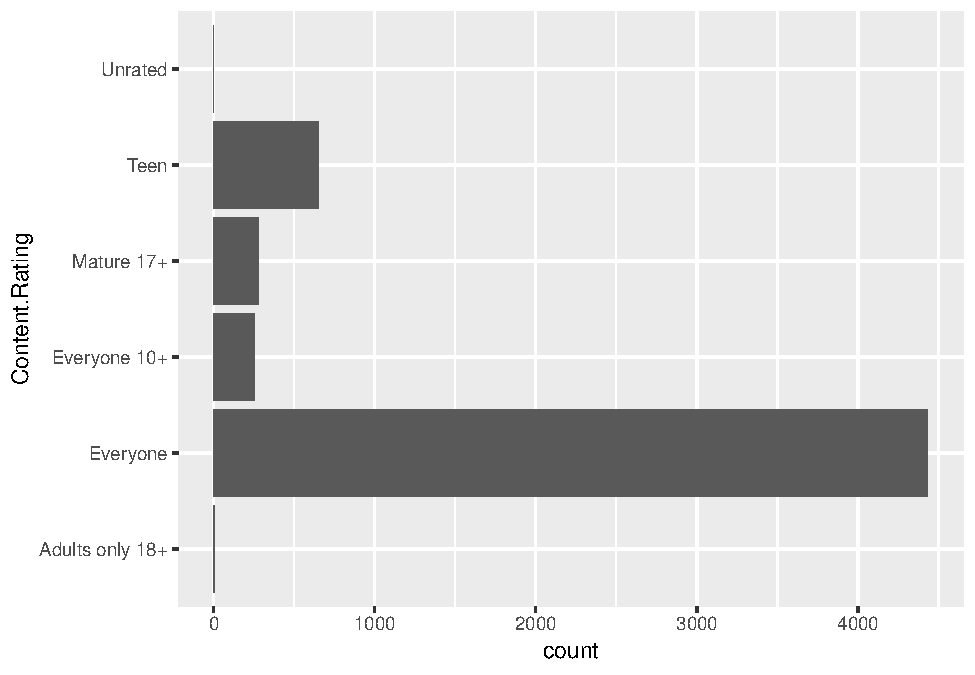
\includegraphics{Project_2_Work_files/figure-latex/unnamed-chunk-15-6.pdf}

Let's look at some of the relationships between the Rating variable, our
response, and some of the possible predictors.

\begin{Shaded}
\begin{Highlighting}[]
\KeywordTok{ggplot}\NormalTok{(Train) +}\StringTok{ }\KeywordTok{geom_boxplot}\NormalTok{(}\KeywordTok{aes}\NormalTok{(}\DataTypeTok{x=}\NormalTok{Category,}\DataTypeTok{y=}\NormalTok{Rating), }\DataTypeTok{fill=}\StringTok{"light green"}\NormalTok{) +}\StringTok{ }\KeywordTok{coord_flip}\NormalTok{()}
\end{Highlighting}
\end{Shaded}

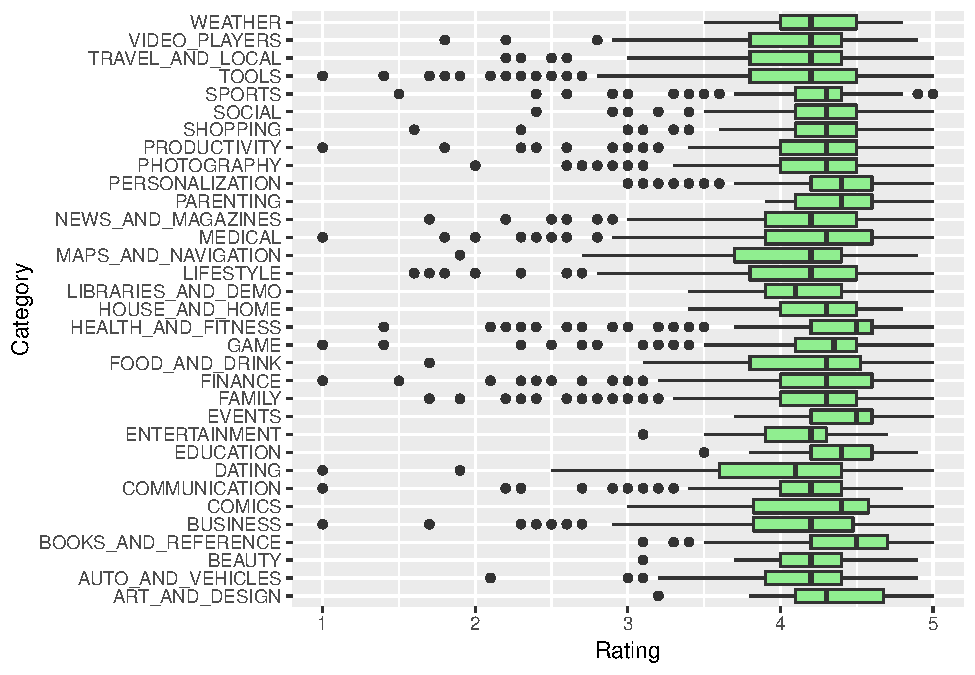
\includegraphics{Project_2_Work_files/figure-latex/unnamed-chunk-16-1.pdf}

\begin{Shaded}
\begin{Highlighting}[]
\KeywordTok{ggplot}\NormalTok{(Train) +}\StringTok{ }\KeywordTok{geom_point}\NormalTok{(}\KeywordTok{aes}\NormalTok{(}\DataTypeTok{x=}\KeywordTok{log}\NormalTok{(Reviews),}\DataTypeTok{y=}\NormalTok{Rating), }\DataTypeTok{color=}\StringTok{"blue"}\NormalTok{)}
\end{Highlighting}
\end{Shaded}

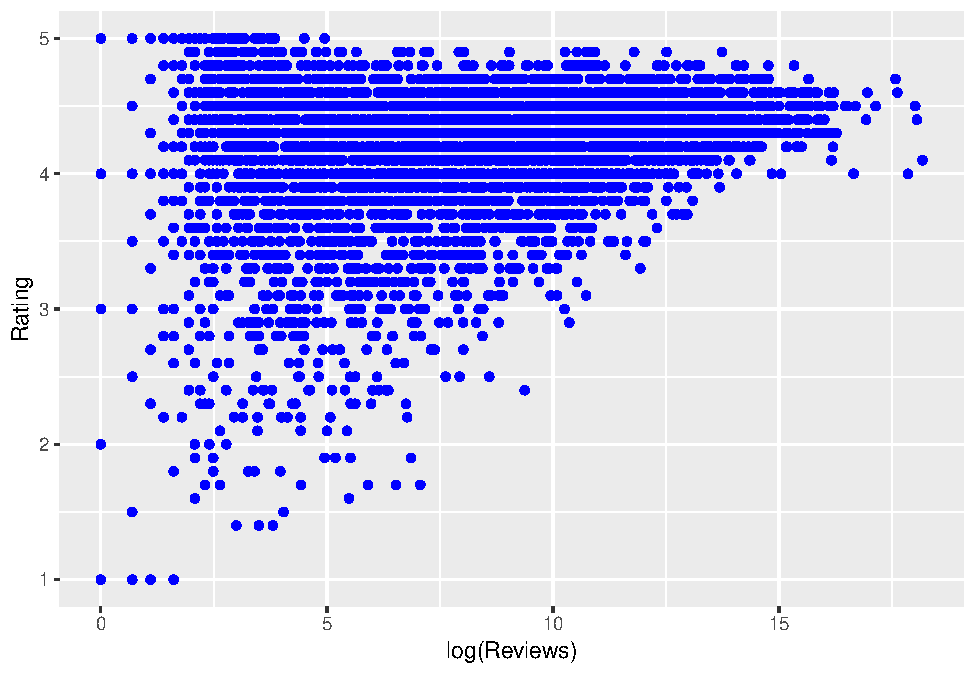
\includegraphics{Project_2_Work_files/figure-latex/unnamed-chunk-16-2.pdf}

\begin{Shaded}
\begin{Highlighting}[]
\KeywordTok{ggplot}\NormalTok{(Train) +}\StringTok{ }\KeywordTok{geom_point}\NormalTok{(}\KeywordTok{aes}\NormalTok{(}\DataTypeTok{x=}\KeywordTok{log}\NormalTok{(Installs),}\DataTypeTok{y=}\NormalTok{Rating), }\DataTypeTok{color=}\StringTok{"purple"}\NormalTok{)}
\end{Highlighting}
\end{Shaded}

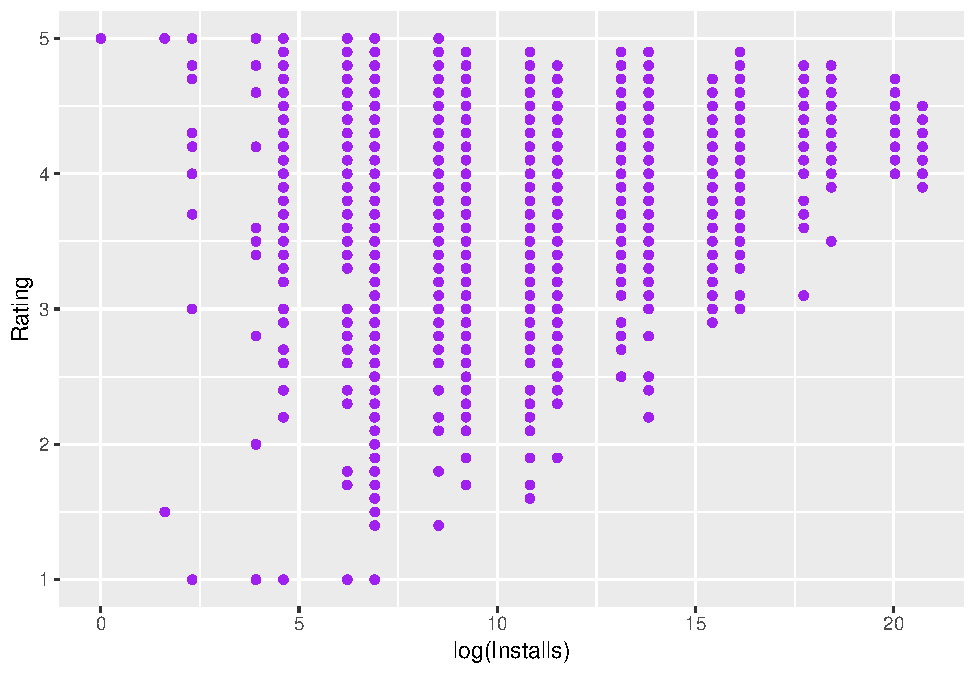
\includegraphics{Project_2_Work_files/figure-latex/unnamed-chunk-16-3.pdf}

\begin{Shaded}
\begin{Highlighting}[]
\KeywordTok{ggplot}\NormalTok{(Train) +}\StringTok{ }\KeywordTok{geom_point}\NormalTok{(}\KeywordTok{aes}\NormalTok{(}\DataTypeTok{x=}\KeywordTok{log}\NormalTok{(Price),}\DataTypeTok{y=}\NormalTok{Rating), }\DataTypeTok{color=}\StringTok{"red"}\NormalTok{)}
\end{Highlighting}
\end{Shaded}

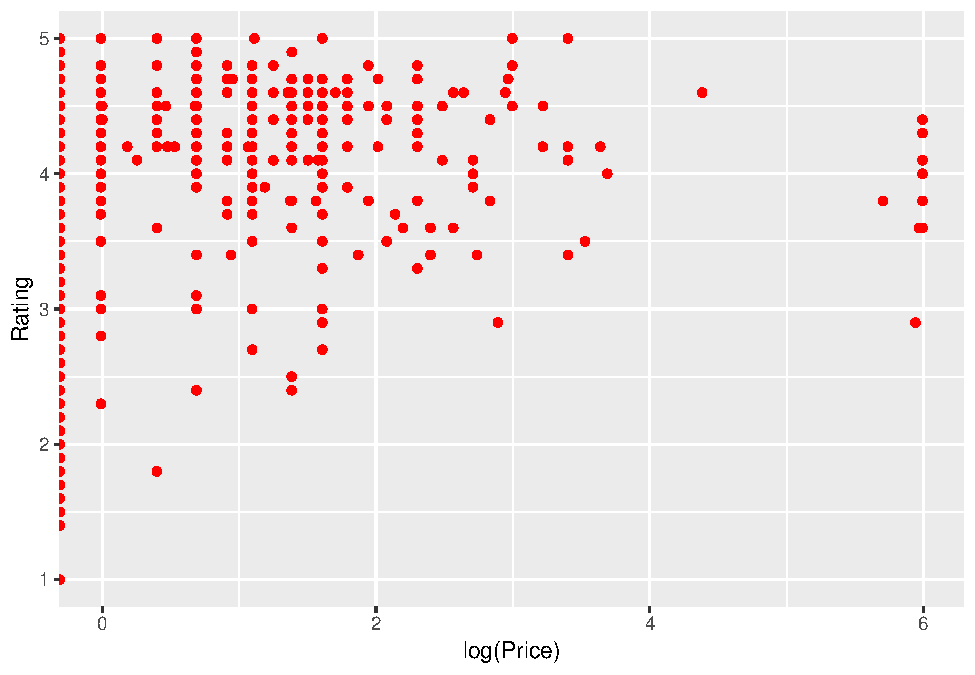
\includegraphics{Project_2_Work_files/figure-latex/unnamed-chunk-16-4.pdf}

\begin{Shaded}
\begin{Highlighting}[]
\KeywordTok{ggplot}\NormalTok{(Train) +}\StringTok{ }\KeywordTok{geom_violin}\NormalTok{(}\KeywordTok{aes}\NormalTok{(}\DataTypeTok{x=}\NormalTok{Content.Rating,}\DataTypeTok{y=}\NormalTok{Rating), }\DataTypeTok{trim=}\OtherTok{FALSE}\NormalTok{, }\DataTypeTok{fill=}\StringTok{"light blue"}\NormalTok{)}
\end{Highlighting}
\end{Shaded}

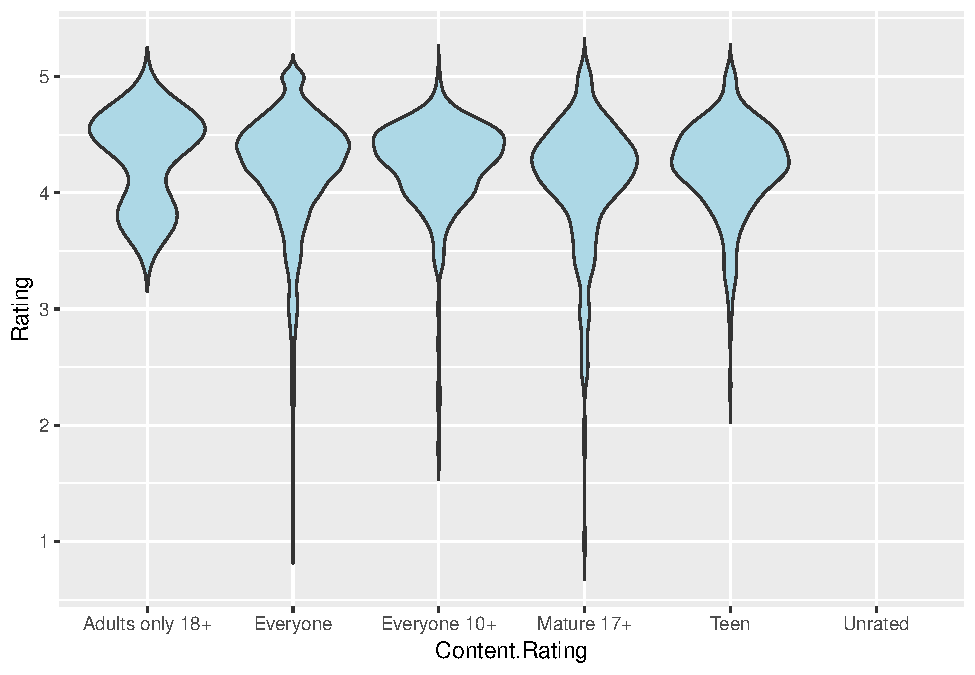
\includegraphics{Project_2_Work_files/figure-latex/unnamed-chunk-16-5.pdf}

Now, let's look at some of the relationships between the other
variables.

\begin{Shaded}
\begin{Highlighting}[]
\KeywordTok{ggplot}\NormalTok{(Train) +}\StringTok{ }\KeywordTok{geom_boxplot}\NormalTok{(}\KeywordTok{aes}\NormalTok{(}\DataTypeTok{x=}\NormalTok{Content.Rating,}\DataTypeTok{y=}\KeywordTok{log}\NormalTok{(Installs)), }\DataTypeTok{fill=}\StringTok{"light green"}\NormalTok{)}
\end{Highlighting}
\end{Shaded}

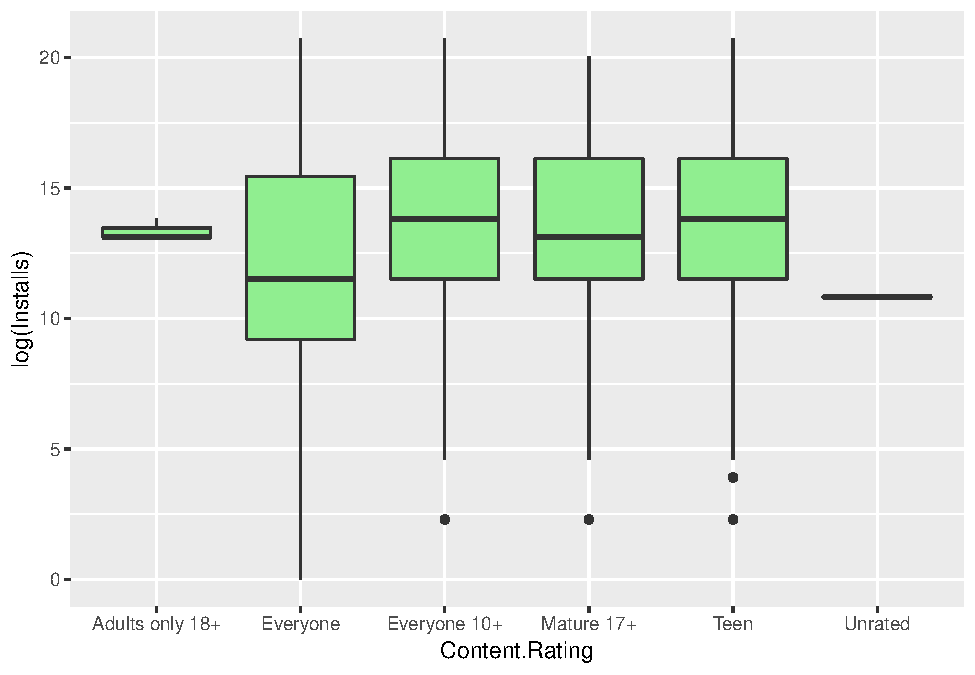
\includegraphics{Project_2_Work_files/figure-latex/unnamed-chunk-17-1.pdf}

\begin{Shaded}
\begin{Highlighting}[]
\KeywordTok{ggplot}\NormalTok{(Train) +}\StringTok{ }\KeywordTok{geom_point}\NormalTok{(}\KeywordTok{aes}\NormalTok{(}\DataTypeTok{x=}\KeywordTok{log}\NormalTok{(Price),}\DataTypeTok{y=}\KeywordTok{log}\NormalTok{(Installs)), }\DataTypeTok{color=}\StringTok{"blue"}\NormalTok{)}
\end{Highlighting}
\end{Shaded}

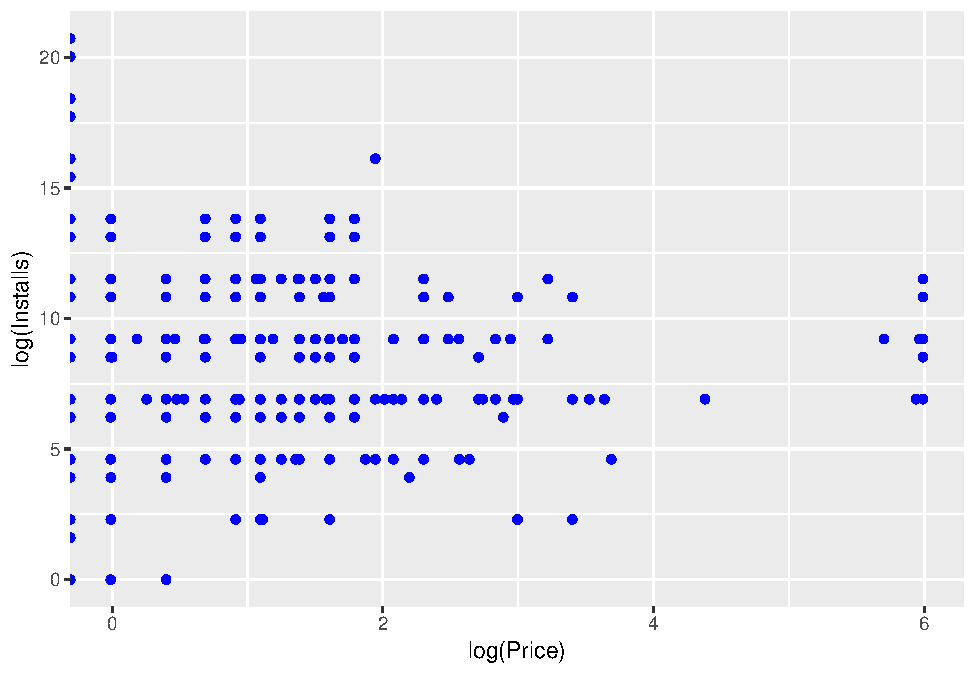
\includegraphics{Project_2_Work_files/figure-latex/unnamed-chunk-17-2.pdf}

\section{Conclusion}\label{conclusion}

It appears from the data that the Reviews variable seems quite
positively related to the Ratings variable. While ratings of 5 can be
achieved across all Review amounts, they seem to be more common with
higher Review amounts. The same can be said for the Installs variable,
in that the more installations a particular app receives could correlate
to the rating it is given. The Price appears to have essentially the
opposite effect. With the exception of free apps, lower priced apps
appear to earn higher rating scores thant more expensive apps. Content
rating does not appear to affect an app's rating.

With regard to the other relationships explored, Content Rating seemd
very equal across app installations, with apps rated as Everyone had the
most variance, probably due to the fact that most of the apps in the
data set are rated Everyone, as seen by the Content Rating bar plot
earlier. When price was compared to installations, an almost bubble
appeared in the bottom right portion of the plot, indicating that less
expensive apps might warrent more installations from users.

Moving forward, we feel that the model we are aiming to create should
include the Review, Installs, and Price variables, possibly Genres and
Category as well.

\section{Questions to Answer in This
Study}\label{questions-to-answer-in-this-study}

\subsection{Broad Questions}\label{broad-questions}

\subsubsection{What makes a good app?}\label{what-makes-a-good-app}

We are interested in seeing what attributes or characteristics, if any,
of a particular app affect how ``good'' it is. Now, ``good'' is a highly
subjective term and with the variety of apps that exist out there, we
cannot generalize them into a category of ``good'' and ``bad''. However,
for the purposes of our look into this matter, we will be defining the
``good''-ness of an app by its rating on a 5 point scale. This allows us
to quantify, to some degree of accuracy, how installers felt about their
experience with the app.

\subsubsection{Can we know in advance if an app will be
good?}\label{can-we-know-in-advance-if-an-app-will-be-good}

This question is the other side of the coin to the previous question.
Basically, if we know certain characteristics about an app, like genre,
price, or content rating, then we can determine how well it will be
rated by installers. We would like to know if this can be done with any
of the variables in our data set.

\subsection{Narrow Questions}\label{narrow-questions}

\subsubsection{Can we create a model that accurately predicts an app's
user rating based on the number of reviews, number of installations,
price, and
category?}\label{can-we-create-a-model-that-accurately-predicts-an-apps-user-rating-based-on-the-number-of-reviews-number-of-installations-price-and-category}

After exploring the data set, we found the number of reviews, number of
installations, and price to have a somewhat apparent correlation with
the app's user rating. Now, we would like to see if a model can
accurately predict that rating while using those variables.

\subsubsection{Can we create a model that accurately predicts and app's
user rating based purely on variables that would be known before the app
is released, such as content rating, price, and
category?}\label{can-we-create-a-model-that-accurately-predicts-and-apps-user-rating-based-purely-on-variables-that-would-be-known-before-the-app-is-released-such-as-content-rating-price-and-category}

This question is an attempt to work with the second broad question,
looking purely at information about an app that does not require user
data. Such a model would be useful for app developers that wish to have
some idea at an app's success before it hits the market. This could
guide their decisions on what apps to support, develop, and market.

\subsection{Discussion}\label{discussion}

We will be creating two predictive models for our data set to hopefully
predict the user rating. The first will be based on the number of
reviews, number of installations, price, and category, and is hoping to
just get a model that is accurate for both the train and test data. The
second model will be based solely on non-user information, such as
content rating, category, and price, and will hopefully be able to
provide accurate predictions for both the train and test data.

\section{Modeling/Hypothesis Testing}\label{modelinghypothesis-testing}

\subsection{Model 1 Unconditional Model
Building}\label{model-1-unconditional-model-building}

\subsubsection{Model 1.A Random Forest}\label{model-1.a-random-forest}

\begin{Shaded}
\begin{Highlighting}[]
\KeywordTok{library}\NormalTok{(randomForest)}
\KeywordTok{set.seed}\NormalTok{(}\DecValTok{42}\NormalTok{)}
\NormalTok{Model1.A <-}\StringTok{ }\KeywordTok{randomForest}\NormalTok{(}\KeywordTok{I}\NormalTok{(}\KeywordTok{log}\NormalTok{(Rating)) ~}\StringTok{ }\NormalTok{Reviews +}\StringTok{ }\NormalTok{Installs +}\StringTok{ }\NormalTok{Price +}\StringTok{ }\NormalTok{Category, }\DataTypeTok{data =} \NormalTok{Train, }\DataTypeTok{mtry =} \DecValTok{4}\NormalTok{)}
\NormalTok{Model1.A.Prediction <-}\StringTok{ }\KeywordTok{predict}\NormalTok{(Model1.A)}
\KeywordTok{plot}\NormalTok{(}\KeywordTok{log}\NormalTok{(Train$Rating),Model1.A.Prediction)}
\KeywordTok{abline}\NormalTok{(}\DecValTok{0}\NormalTok{,}\DecValTok{1}\NormalTok{,}\DataTypeTok{col=}\StringTok{"red"}\NormalTok{)}
\end{Highlighting}
\end{Shaded}

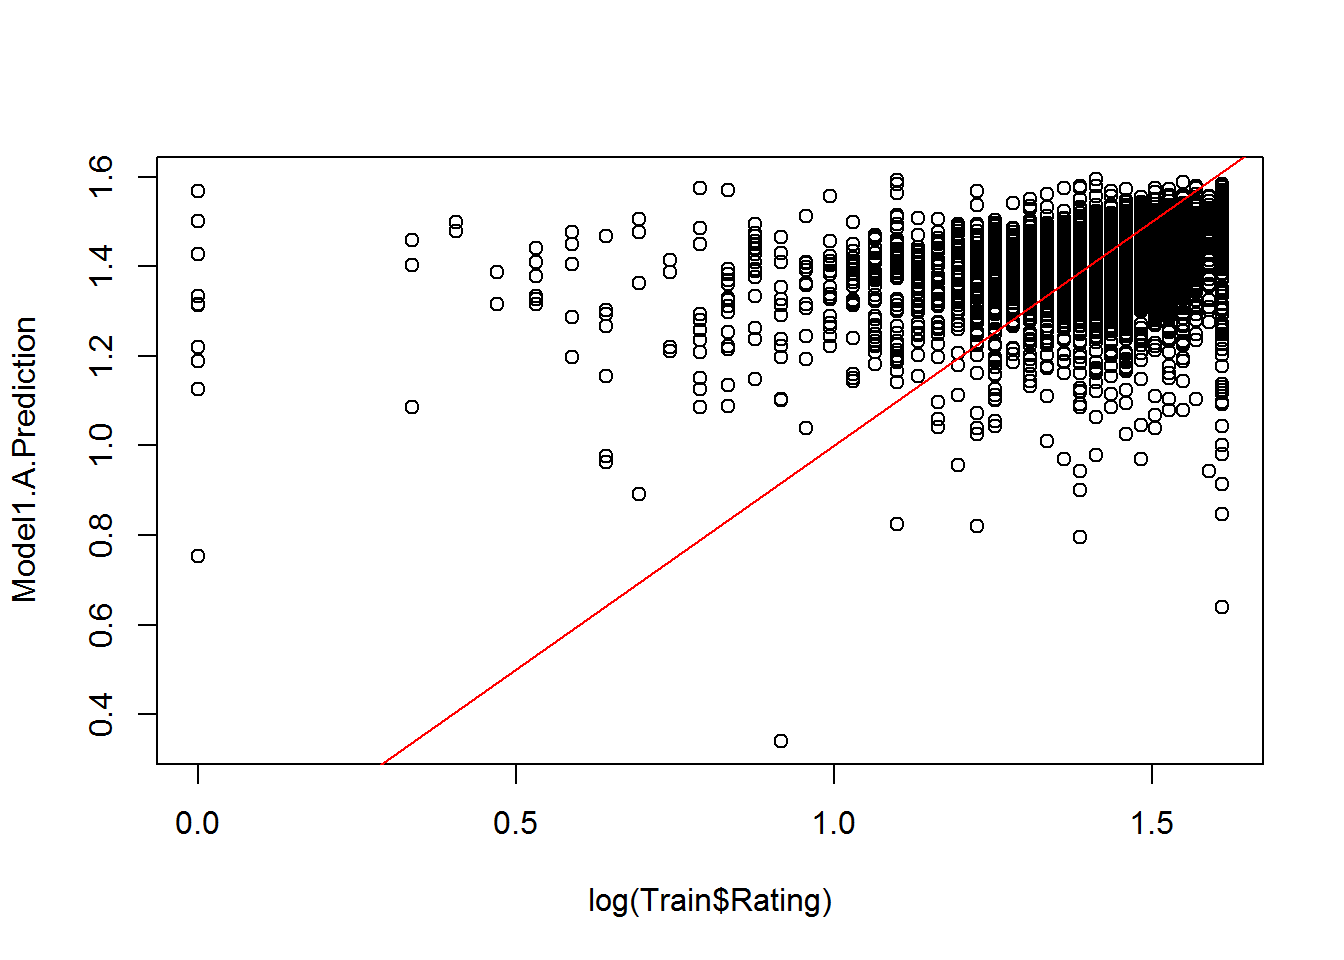
\includegraphics{Project_2_Work_files/figure-latex/unnamed-chunk-18-1.pdf}

This random forest model incorporates the number of reviews, the price,
the number of installations, and the category of the app in an effort to
predict the rating. The plot seen above shows the predictions with the
line in red showing where the prediction and the rating are equal. As a
note, for the creation of the model, the log(Rating) was used so the
plot reflects that, as doing that more evenly distributed the scores. As
can be seen by the plot, the model over estimates lower user rating
scores.

\begin{Shaded}
\begin{Highlighting}[]
\NormalTok{Test <-}\StringTok{ }\KeywordTok{read.csv}\NormalTok{(}\StringTok{"Test.csv"}\NormalTok{)}
\KeywordTok{levels}\NormalTok{(Test$Category) <-}\StringTok{ }\KeywordTok{levels}\NormalTok{(Train$Category)}
\NormalTok{Model1.A.Prediction.Test <-}\StringTok{ }\KeywordTok{predict}\NormalTok{(Model1.A,}\DataTypeTok{newdata=}\NormalTok{Test)}
\KeywordTok{plot}\NormalTok{(}\KeywordTok{log}\NormalTok{(Test$Rating),Model1.A.Prediction.Test)}
\KeywordTok{abline}\NormalTok{(}\DecValTok{0}\NormalTok{,}\DecValTok{1}\NormalTok{,}\DataTypeTok{col=}\StringTok{"red"}\NormalTok{)}
\end{Highlighting}
\end{Shaded}

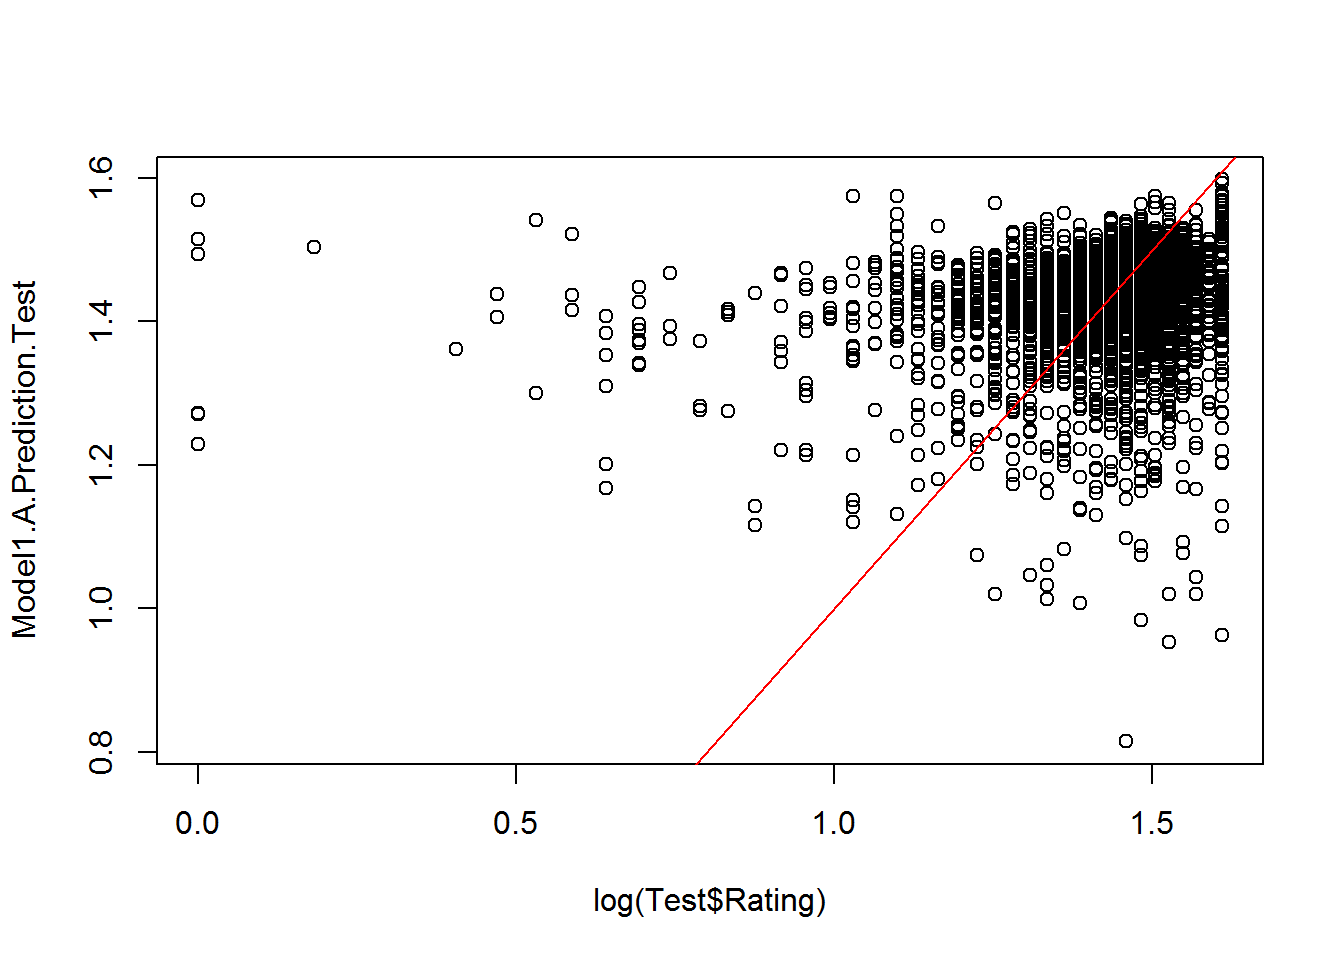
\includegraphics{Project_2_Work_files/figure-latex/unnamed-chunk-19-1.pdf}

\begin{Shaded}
\begin{Highlighting}[]
\KeywordTok{rm}\NormalTok{(Test)}
\end{Highlighting}
\end{Shaded}

Oddly enough, at first glance, the model appears to perform slightly
better with the test data, but still overestimates low user rating
scores; however, it can be seen this model, while not glowingly
accurate, does not perform diffently with never before seen data.

\subsubsection{Model 1.B Linear Model}\label{model-1.b-linear-model}

\begin{Shaded}
\begin{Highlighting}[]
\NormalTok{Model1.B <-}\StringTok{ }\KeywordTok{lm}\NormalTok{(Rating ~}\StringTok{ }\KeywordTok{I}\NormalTok{(}\KeywordTok{log}\NormalTok{(Reviews)) +}\StringTok{ }\KeywordTok{I}\NormalTok{(}\KeywordTok{log}\NormalTok{(Installs)) +}\StringTok{ }\NormalTok{Price +}\StringTok{ }\NormalTok{Category, }\DataTypeTok{data=}\NormalTok{Train)}
\NormalTok{Model1.B.Prediction <-}\StringTok{ }\KeywordTok{predict}\NormalTok{(Model1.B)}
\KeywordTok{summary}\NormalTok{(Model1.B)}
\end{Highlighting}
\end{Shaded}

\begin{verbatim}
## 
## Call:
## lm(formula = Rating ~ I(log(Reviews)) + I(log(Installs)) + Price + 
##     Category, data = Train)
## 
## Residuals:
##     Min      1Q  Median      3Q     Max 
## -3.0780 -0.1784  0.0500  0.2682  1.3745 
## 
## Coefficients:
##                               Estimate Std. Error t value Pr(>|t|)    
## (Intercept)                  4.7824237  0.0887919  53.861  < 2e-16 ***
## I(log(Reviews))              0.1590634  0.0059847  26.578  < 2e-16 ***
## I(log(Installs))            -0.1351149  0.0060001 -22.519  < 2e-16 ***
## Price                       -0.0010287  0.0003742  -2.749 0.005988 ** 
## CategoryAUTO_AND_VEHICLES   -0.2597760  0.1117275  -2.325 0.020103 *  
## CategoryBEAUTY              -0.0836898  0.1196155  -0.700 0.484171    
## CategoryBOOKS_AND_REFERENCE -0.0441487  0.0962096  -0.459 0.646338    
## CategoryBUSINESS            -0.2985174  0.0902341  -3.308 0.000945 ***
## CategoryCOMICS              -0.2554503  0.1111951  -2.297 0.021638 *  
## CategoryCOMMUNICATION       -0.3639872  0.0896132  -4.062 4.94e-05 ***
## CategoryDATING              -0.4795769  0.0935859  -5.124 3.08e-07 ***
## CategoryEDUCATION           -0.1116429  0.0967430  -1.154 0.248544    
## CategoryENTERTAINMENT       -0.3733013  0.0969719  -3.850 0.000120 ***
## CategoryEVENTS               0.0969359  0.1242322   0.780 0.435259    
## CategoryFAMILY              -0.2292887  0.0840470  -2.728 0.006390 ** 
## CategoryFINANCE             -0.2579701  0.0896630  -2.877 0.004029 ** 
## CategoryFOOD_AND_DRINK      -0.2572679  0.1047934  -2.455 0.014119 *  
## CategoryGAME                -0.2909103  0.0852579  -3.412 0.000649 ***
## CategoryHEALTH_AND_FITNESS  -0.2187885  0.0894152  -2.447 0.014440 *  
## CategoryHOUSE_AND_HOME      -0.2125849  0.1067025  -1.992 0.046385 *  
## CategoryLIBRARIES_AND_DEMO  -0.1725551  0.1137155  -1.517 0.129215    
## CategoryLIFESTYLE           -0.3032571  0.0899269  -3.372 0.000751 ***
## CategoryMAPS_AND_NAVIGATION -0.4123675  0.1002973  -4.111 3.99e-05 ***
## CategoryMEDICAL             -0.1924384  0.0893484  -2.154 0.031299 *  
## CategoryNEWS_AND_MAGAZINES  -0.3592561  0.0919499  -3.907 9.45e-05 ***
## CategoryPARENTING            0.0861430  0.1300361   0.662 0.507707    
## CategoryPERSONALIZATION     -0.1156563  0.0898918  -1.287 0.198282    
## CategoryPHOTOGRAPHY         -0.2624715  0.0896624  -2.927 0.003433 ** 
## CategoryPRODUCTIVITY        -0.2243243  0.0893940  -2.509 0.012122 *  
## CategorySHOPPING            -0.2590566  0.0939940  -2.756 0.005869 ** 
## CategorySOCIAL              -0.2580975  0.0914772  -2.821 0.004798 ** 
## CategorySPORTS              -0.2977191  0.0894411  -3.329 0.000878 ***
## CategoryTOOLS               -0.3426418  0.0856729  -3.999 6.43e-05 ***
## CategoryTRAVEL_AND_LOCAL    -0.3573351  0.0926315  -3.858 0.000116 ***
## CategoryVIDEO_PLAYERS       -0.3702765  0.0973459  -3.804 0.000144 ***
## CategoryWEATHER             -0.2606247  0.1056110  -2.468 0.013625 *  
## ---
## Signif. codes:  0 '***' 0.001 '**' 0.01 '*' 0.05 '.' 0.1 ' ' 1
## 
## Residual standard error: 0.4816 on 5584 degrees of freedom
## Multiple R-squared:  0.1559, Adjusted R-squared:  0.1506 
## F-statistic: 29.47 on 35 and 5584 DF,  p-value: < 2.2e-16
\end{verbatim}

\begin{Shaded}
\begin{Highlighting}[]
\KeywordTok{plot}\NormalTok{(Train$Rating,Model1.B.Prediction)}
\KeywordTok{abline}\NormalTok{(}\DecValTok{0}\NormalTok{,}\DecValTok{1}\NormalTok{,}\DataTypeTok{col=}\StringTok{"red"}\NormalTok{)}
\end{Highlighting}
\end{Shaded}

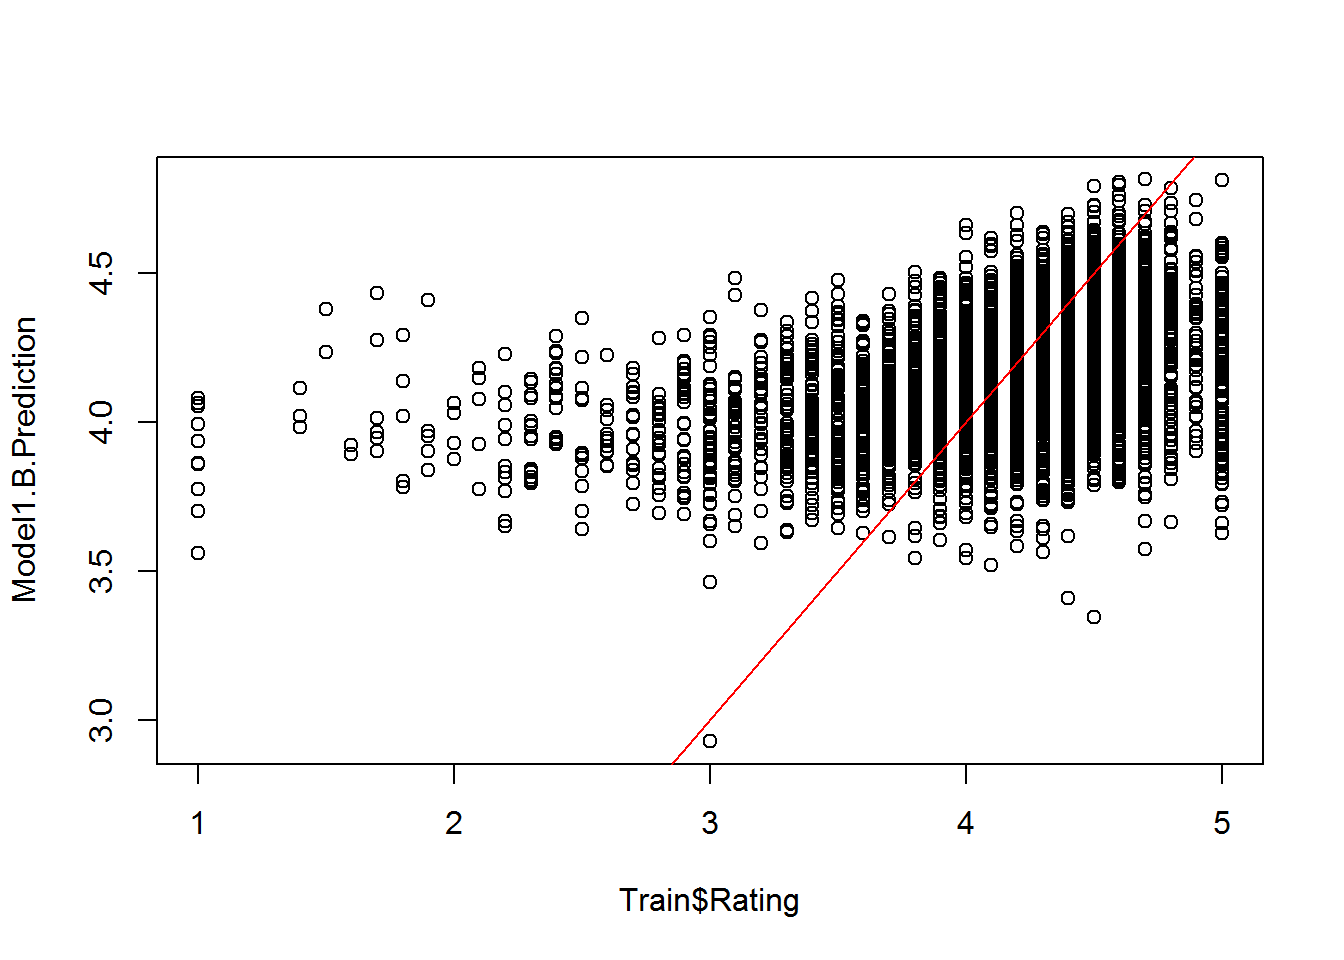
\includegraphics{Project_2_Work_files/figure-latex/unnamed-chunk-20-1.pdf}

This linear model works to predict the rating score with the same
predictor variables as the previous model, and it appears to perform
quite poorly, only fitting the data around 14\%.

\begin{Shaded}
\begin{Highlighting}[]
\NormalTok{Test <-}\StringTok{ }\KeywordTok{read.csv}\NormalTok{(}\StringTok{"Test.csv"}\NormalTok{)}
\NormalTok{Model1.B.Prediction.Test <-}\StringTok{ }\KeywordTok{predict}\NormalTok{(Model1.B,}\DataTypeTok{newdata=}\NormalTok{Test)}
\KeywordTok{plot}\NormalTok{(Test$Rating,Model1.B.Prediction.Test)}
\KeywordTok{abline}\NormalTok{(}\DecValTok{0}\NormalTok{,}\DecValTok{1}\NormalTok{,}\DataTypeTok{col=}\StringTok{"red"}\NormalTok{)}
\end{Highlighting}
\end{Shaded}

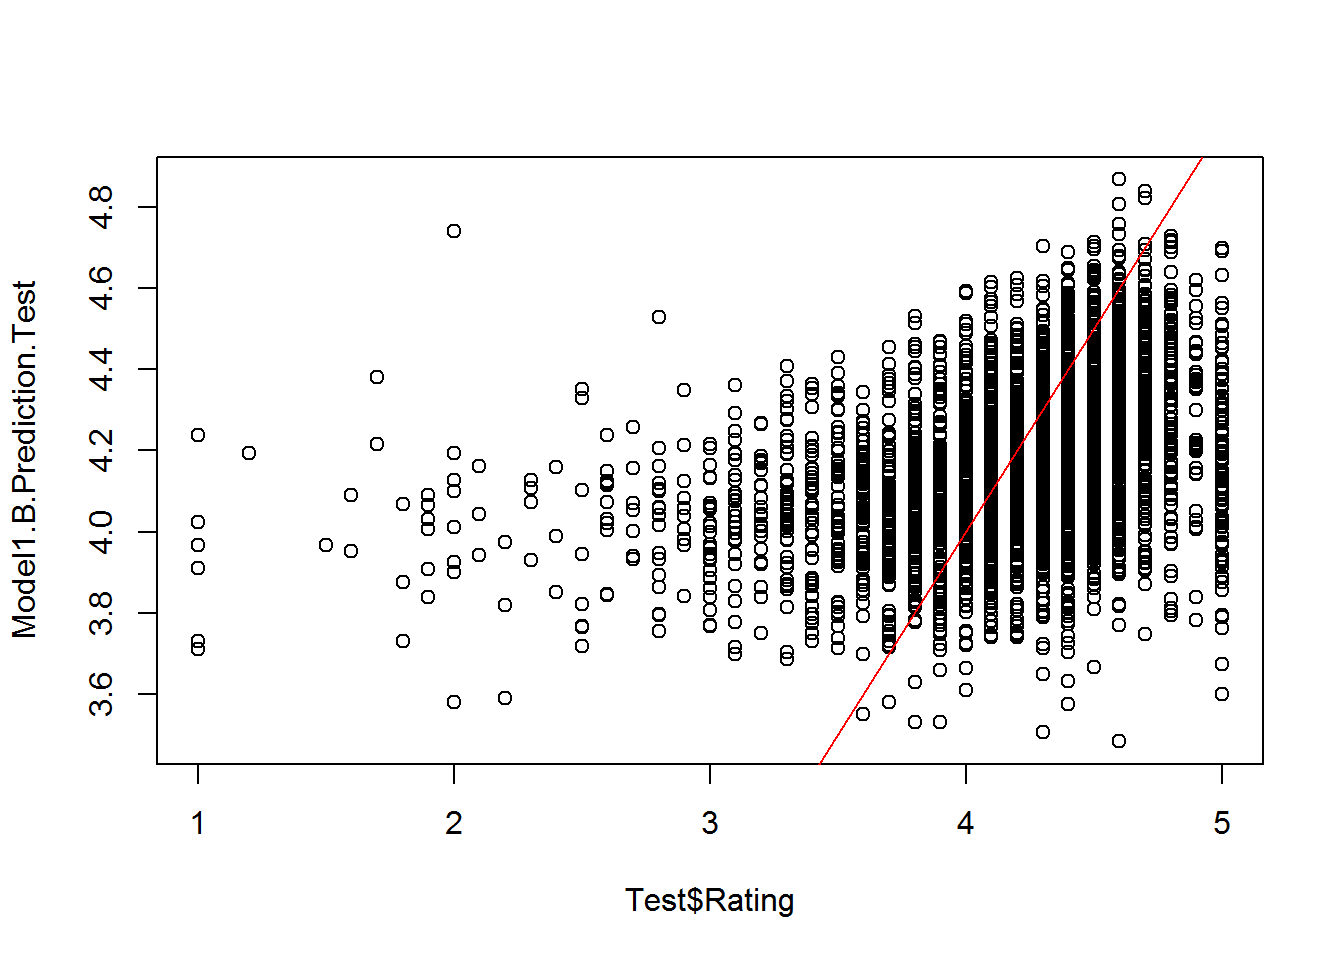
\includegraphics{Project_2_Work_files/figure-latex/unnamed-chunk-21-1.pdf}

\begin{Shaded}
\begin{Highlighting}[]
\KeywordTok{rm}\NormalTok{(Test)}
\end{Highlighting}
\end{Shaded}

The data seems to perform worse for the test data set, indicating that
the linear model slightly over fits the training data and cannot
consistently perform with never before seen data. Overall, this model is
worse than the random forest model discussed previously.

\subsection{Model 2 Non-User Data Model
Building}\label{model-2-non-user-data-model-building}

\subsubsection{Model 2.A Random Forest}\label{model-2.a-random-forest}

\begin{Shaded}
\begin{Highlighting}[]
\KeywordTok{library}\NormalTok{(randomForest)}
\KeywordTok{set.seed}\NormalTok{(}\DecValTok{42}\NormalTok{)}
\NormalTok{Model2.A <-}\StringTok{ }\KeywordTok{randomForest}\NormalTok{(}\KeywordTok{I}\NormalTok{(}\KeywordTok{log}\NormalTok{(Rating)) ~}\StringTok{ }\NormalTok{Price +}\StringTok{ }\NormalTok{Category +}\StringTok{ }\NormalTok{Content.Rating, }\DataTypeTok{data =} \NormalTok{Train, }\DataTypeTok{mtry =} \DecValTok{3}\NormalTok{)}
\NormalTok{Model2.A.Prediction <-}\StringTok{ }\KeywordTok{predict}\NormalTok{(Model2.A)}
\KeywordTok{plot}\NormalTok{(}\KeywordTok{log}\NormalTok{(Train$Rating),Model2.A.Prediction)}
\KeywordTok{abline}\NormalTok{(}\DecValTok{0}\NormalTok{,}\DecValTok{1}\NormalTok{,}\DataTypeTok{col=}\StringTok{"red"}\NormalTok{)}
\end{Highlighting}
\end{Shaded}

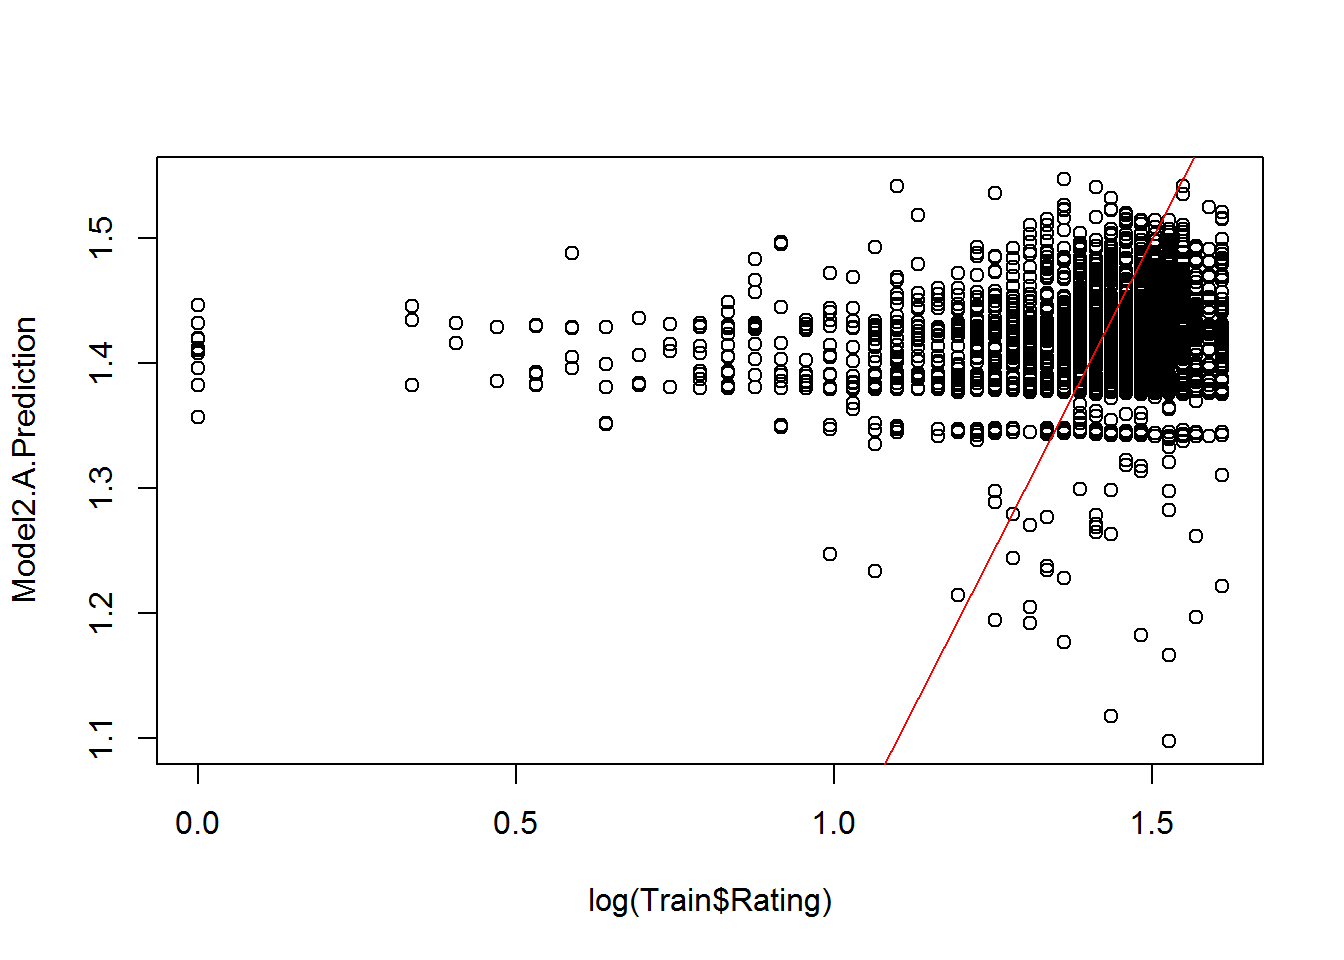
\includegraphics{Project_2_Work_files/figure-latex/unnamed-chunk-22-1.pdf}

Here, we have a random forest model similar to that of Model 1.A, with
the only exception being that it is based upon the data that can be
gathered before the app is relased to the public, price, category, and
content rating. Much like in all of the other models, this one also
overestimates lower user ratings.

\begin{Shaded}
\begin{Highlighting}[]
\NormalTok{Test <-}\StringTok{ }\KeywordTok{read.csv}\NormalTok{(}\StringTok{"Test.csv"}\NormalTok{)}
\KeywordTok{levels}\NormalTok{(Test$Category) <-}\StringTok{ }\KeywordTok{levels}\NormalTok{(Train$Category)}
\KeywordTok{levels}\NormalTok{(Test$Content.Rating) <-}\StringTok{ }\KeywordTok{levels}\NormalTok{(Train$Content.Rating)}
\NormalTok{Model2.A.Prediction.Test <-}\StringTok{ }\KeywordTok{predict}\NormalTok{(Model2.A,}\DataTypeTok{newdata=}\NormalTok{Test)}
\KeywordTok{plot}\NormalTok{(}\KeywordTok{log}\NormalTok{(Test$Rating),Model2.A.Prediction.Test)}
\KeywordTok{abline}\NormalTok{(}\DecValTok{0}\NormalTok{,}\DecValTok{1}\NormalTok{,}\DataTypeTok{col=}\StringTok{"red"}\NormalTok{)}
\end{Highlighting}
\end{Shaded}

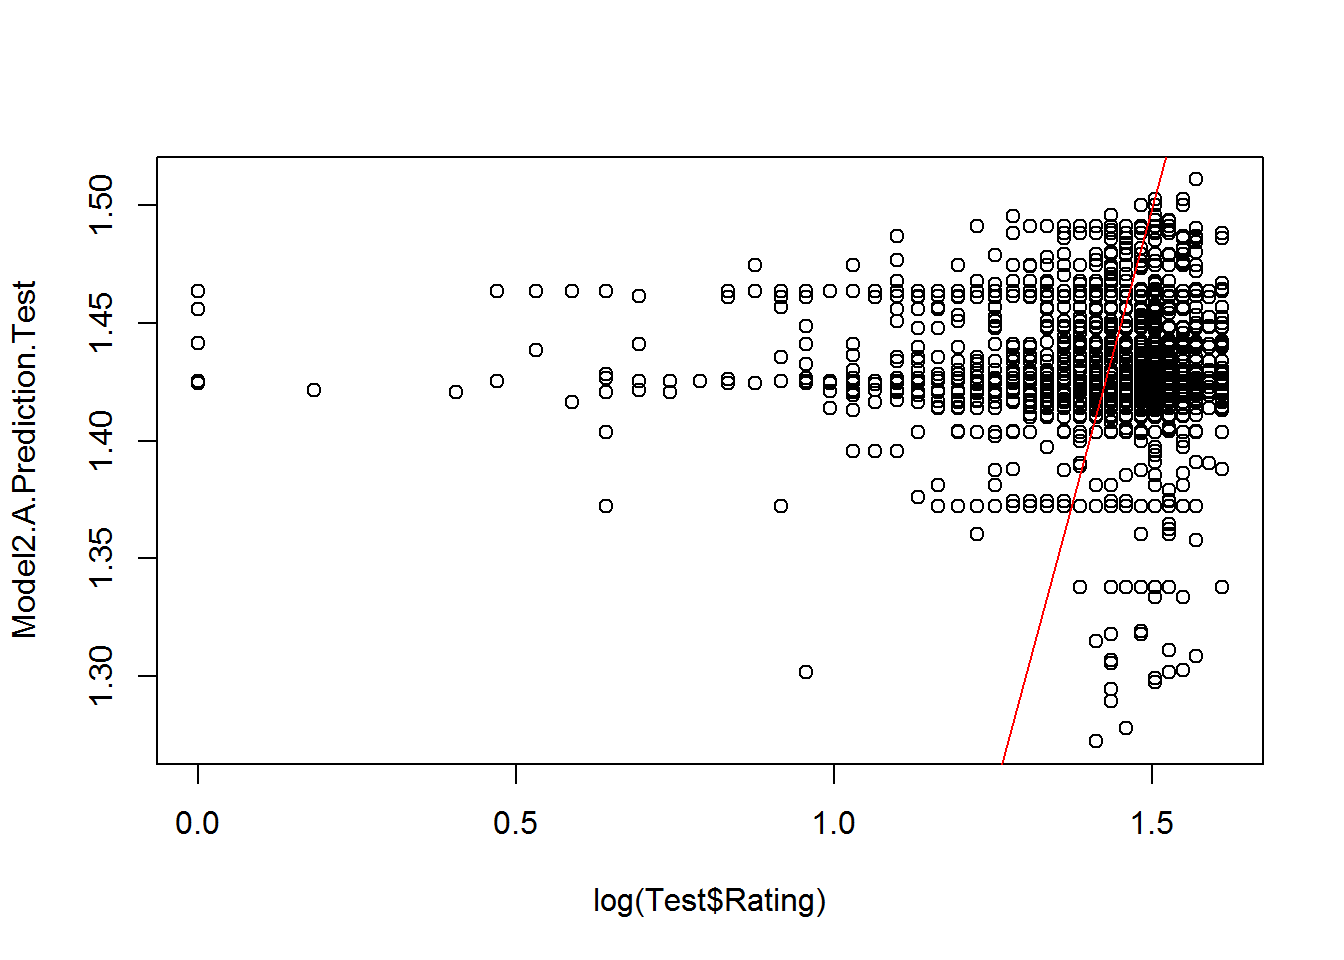
\includegraphics{Project_2_Work_files/figure-latex/unnamed-chunk-23-1.pdf}

\begin{Shaded}
\begin{Highlighting}[]
\KeywordTok{rm}\NormalTok{(Test)}
\end{Highlighting}
\end{Shaded}

Surprisingly, the model appears to perform better on the test data than
it did on the training data. While it still overestimates, lower user
rating scores, it is not as dramatic as with the training data, which is
interesting.

\subsubsection{Model 2.B Linear Model}\label{model-2.b-linear-model}

\begin{Shaded}
\begin{Highlighting}[]
\NormalTok{Model2.B <-}\StringTok{ }\KeywordTok{lm}\NormalTok{(Rating ~}\StringTok{ }\KeywordTok{I}\NormalTok{(}\KeywordTok{log}\NormalTok{(Reviews)) +}\StringTok{ }\KeywordTok{I}\NormalTok{(}\KeywordTok{log}\NormalTok{(Installs)) +}\StringTok{ }\NormalTok{Price +}\StringTok{ }\NormalTok{Category, }\DataTypeTok{data=}\NormalTok{Train)}
\NormalTok{Model2.B.Prediction <-}\StringTok{ }\KeywordTok{predict}\NormalTok{(Model2.B)}
\KeywordTok{summary}\NormalTok{(Model2.B)}
\end{Highlighting}
\end{Shaded}

\begin{verbatim}
## 
## Call:
## lm(formula = Rating ~ I(log(Reviews)) + I(log(Installs)) + Price + 
##     Category, data = Train)
## 
## Residuals:
##     Min      1Q  Median      3Q     Max 
## -3.0780 -0.1784  0.0500  0.2682  1.3745 
## 
## Coefficients:
##                               Estimate Std. Error t value Pr(>|t|)    
## (Intercept)                  4.7824237  0.0887919  53.861  < 2e-16 ***
## I(log(Reviews))              0.1590634  0.0059847  26.578  < 2e-16 ***
## I(log(Installs))            -0.1351149  0.0060001 -22.519  < 2e-16 ***
## Price                       -0.0010287  0.0003742  -2.749 0.005988 ** 
## CategoryAUTO_AND_VEHICLES   -0.2597760  0.1117275  -2.325 0.020103 *  
## CategoryBEAUTY              -0.0836898  0.1196155  -0.700 0.484171    
## CategoryBOOKS_AND_REFERENCE -0.0441487  0.0962096  -0.459 0.646338    
## CategoryBUSINESS            -0.2985174  0.0902341  -3.308 0.000945 ***
## CategoryCOMICS              -0.2554503  0.1111951  -2.297 0.021638 *  
## CategoryCOMMUNICATION       -0.3639872  0.0896132  -4.062 4.94e-05 ***
## CategoryDATING              -0.4795769  0.0935859  -5.124 3.08e-07 ***
## CategoryEDUCATION           -0.1116429  0.0967430  -1.154 0.248544    
## CategoryENTERTAINMENT       -0.3733013  0.0969719  -3.850 0.000120 ***
## CategoryEVENTS               0.0969359  0.1242322   0.780 0.435259    
## CategoryFAMILY              -0.2292887  0.0840470  -2.728 0.006390 ** 
## CategoryFINANCE             -0.2579701  0.0896630  -2.877 0.004029 ** 
## CategoryFOOD_AND_DRINK      -0.2572679  0.1047934  -2.455 0.014119 *  
## CategoryGAME                -0.2909103  0.0852579  -3.412 0.000649 ***
## CategoryHEALTH_AND_FITNESS  -0.2187885  0.0894152  -2.447 0.014440 *  
## CategoryHOUSE_AND_HOME      -0.2125849  0.1067025  -1.992 0.046385 *  
## CategoryLIBRARIES_AND_DEMO  -0.1725551  0.1137155  -1.517 0.129215    
## CategoryLIFESTYLE           -0.3032571  0.0899269  -3.372 0.000751 ***
## CategoryMAPS_AND_NAVIGATION -0.4123675  0.1002973  -4.111 3.99e-05 ***
## CategoryMEDICAL             -0.1924384  0.0893484  -2.154 0.031299 *  
## CategoryNEWS_AND_MAGAZINES  -0.3592561  0.0919499  -3.907 9.45e-05 ***
## CategoryPARENTING            0.0861430  0.1300361   0.662 0.507707    
## CategoryPERSONALIZATION     -0.1156563  0.0898918  -1.287 0.198282    
## CategoryPHOTOGRAPHY         -0.2624715  0.0896624  -2.927 0.003433 ** 
## CategoryPRODUCTIVITY        -0.2243243  0.0893940  -2.509 0.012122 *  
## CategorySHOPPING            -0.2590566  0.0939940  -2.756 0.005869 ** 
## CategorySOCIAL              -0.2580975  0.0914772  -2.821 0.004798 ** 
## CategorySPORTS              -0.2977191  0.0894411  -3.329 0.000878 ***
## CategoryTOOLS               -0.3426418  0.0856729  -3.999 6.43e-05 ***
## CategoryTRAVEL_AND_LOCAL    -0.3573351  0.0926315  -3.858 0.000116 ***
## CategoryVIDEO_PLAYERS       -0.3702765  0.0973459  -3.804 0.000144 ***
## CategoryWEATHER             -0.2606247  0.1056110  -2.468 0.013625 *  
## ---
## Signif. codes:  0 '***' 0.001 '**' 0.01 '*' 0.05 '.' 0.1 ' ' 1
## 
## Residual standard error: 0.4816 on 5584 degrees of freedom
## Multiple R-squared:  0.1559, Adjusted R-squared:  0.1506 
## F-statistic: 29.47 on 35 and 5584 DF,  p-value: < 2.2e-16
\end{verbatim}

\begin{Shaded}
\begin{Highlighting}[]
\KeywordTok{plot}\NormalTok{(Train$Rating,Model2.B.Prediction)}
\KeywordTok{abline}\NormalTok{(}\DecValTok{0}\NormalTok{,}\DecValTok{1}\NormalTok{,}\DataTypeTok{col=}\StringTok{"red"}\NormalTok{)}
\end{Highlighting}
\end{Shaded}

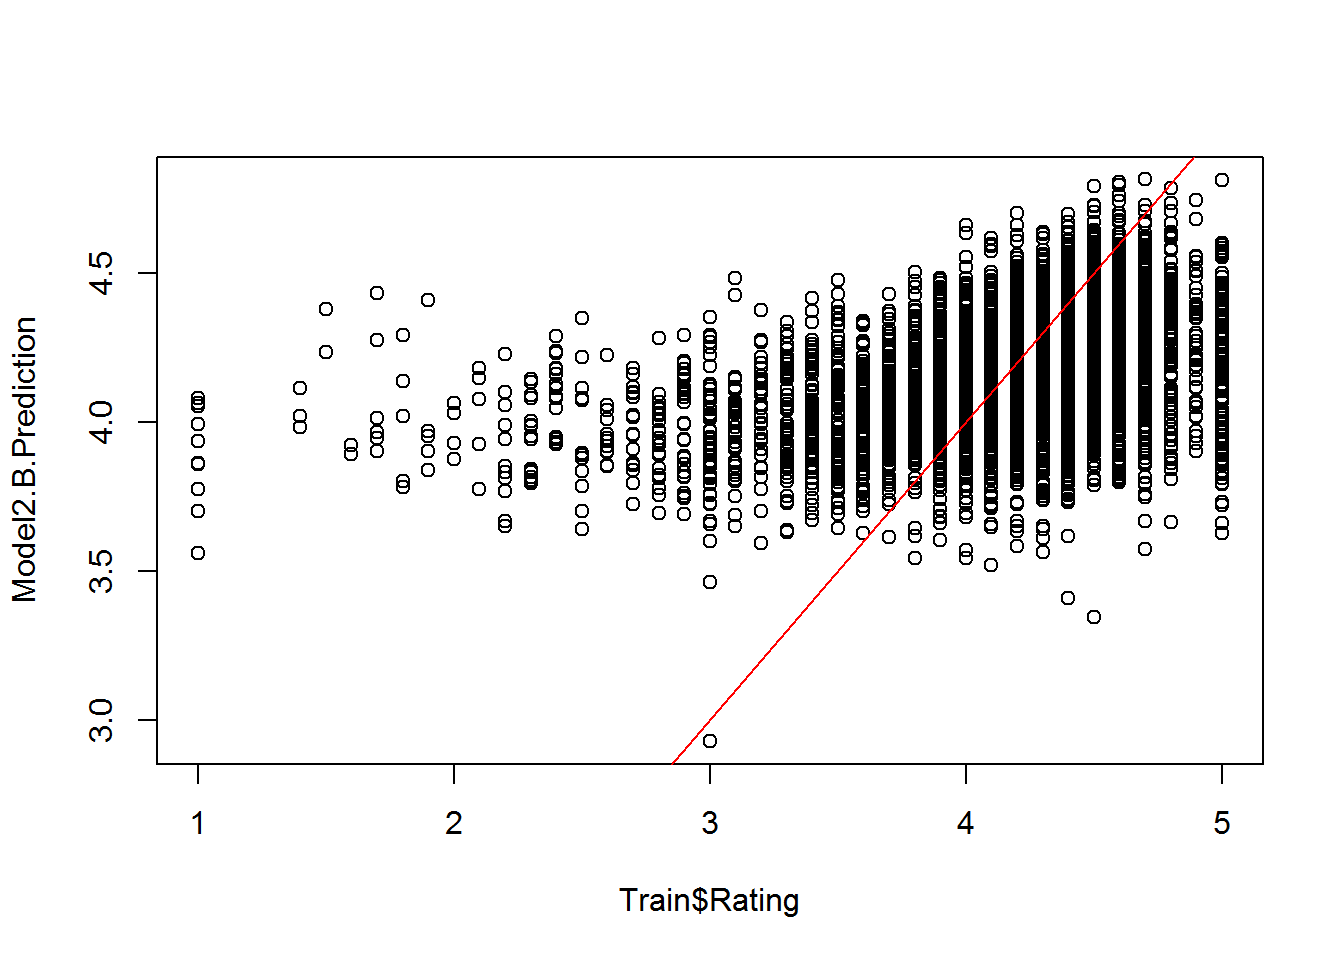
\includegraphics{Project_2_Work_files/figure-latex/unnamed-chunk-24-1.pdf}

This model is depressingly inaccurate, and drastically overestimates
lower user rating scores. It is a linear model based on the same
predictors as Model2.A. Much like Model1.A, it only fits the data about
15\%.

\begin{Shaded}
\begin{Highlighting}[]
\NormalTok{Test <-}\StringTok{ }\KeywordTok{read.csv}\NormalTok{(}\StringTok{"Test.csv"}\NormalTok{)}
\NormalTok{Model2.B.Prediction.Test <-}\StringTok{ }\KeywordTok{predict}\NormalTok{(Model2.B,}\DataTypeTok{newdata=}\NormalTok{Test)}
\KeywordTok{plot}\NormalTok{(Test$Rating,Model2.B.Prediction.Test)}
\KeywordTok{abline}\NormalTok{(}\DecValTok{0}\NormalTok{,}\DecValTok{1}\NormalTok{,}\DataTypeTok{col=}\StringTok{"red"}\NormalTok{)}
\end{Highlighting}
\end{Shaded}

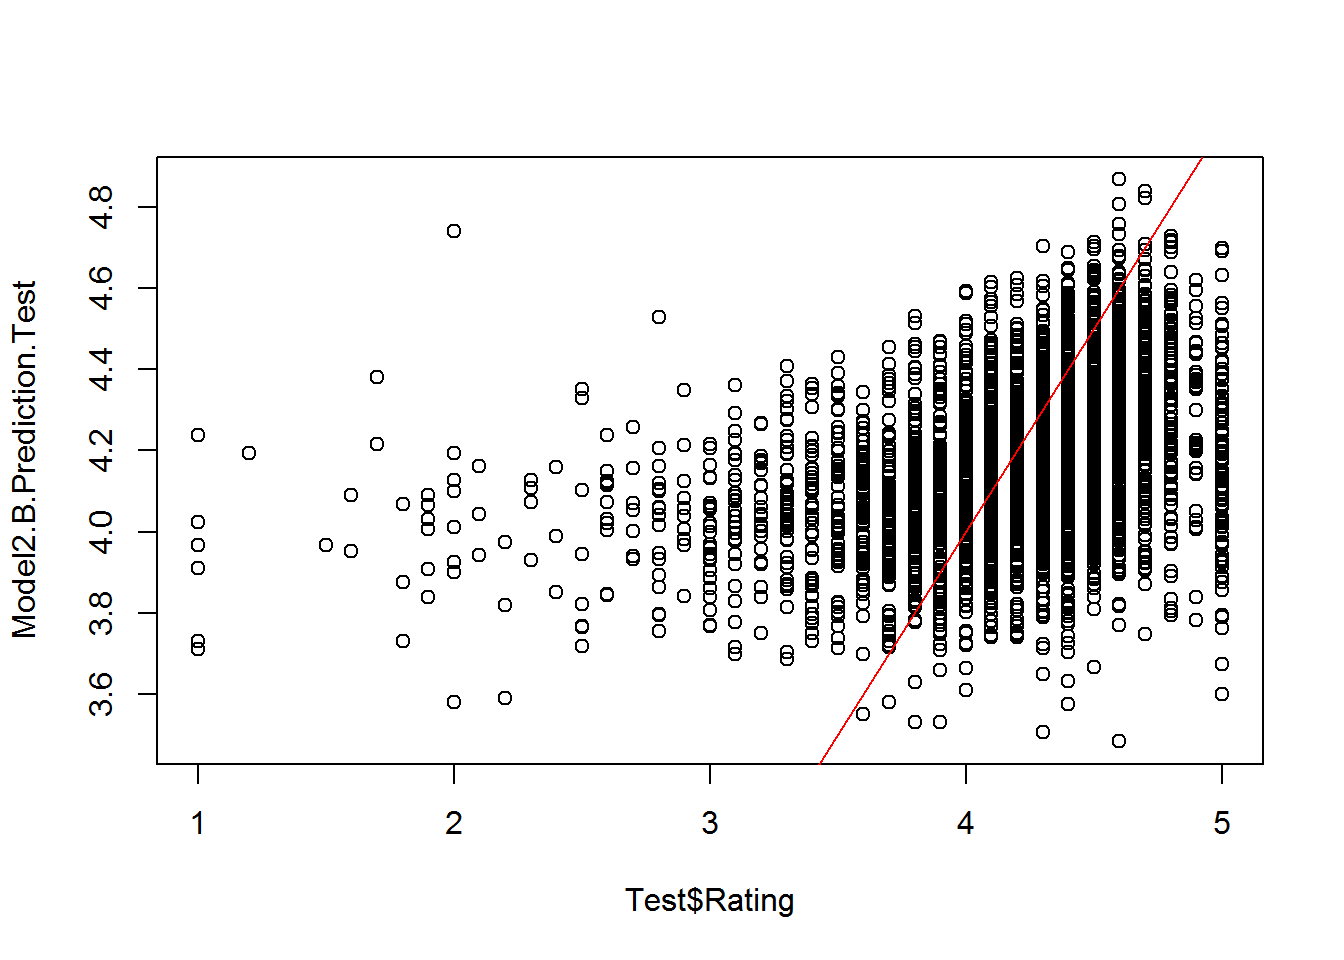
\includegraphics{Project_2_Work_files/figure-latex/unnamed-chunk-25-1.pdf}

\begin{Shaded}
\begin{Highlighting}[]
\KeywordTok{rm}\NormalTok{(Test)}
\end{Highlighting}
\end{Shaded}

The model performs worse when tested against the test data than to the
training data. This indicates that, as poor as the model fit the
training data, it is overfitting the data and is not generalizing all of
the data well. It overestimates the lower user rating scores quite a
bit.

\section{Results}\label{results}

It was determined when the models were built and tested that the Random
Forest models were superior to the linear models. This determination was
based on how close the data points were to the y=x line on the plots,
and how many drastic points there were. This decision was also based on
the performance of the models on the test data, in which the Random
Forest models performed as well, if not, better, than on the training
dat while the linear model was not able to generalize the data to a
satisfactory degree. There were two final models that were developed.
Model1A, a random forest model, incorporated the Category, Reviews,
Installs, and Price variables in order to predict the log of the Rating
variable. Its purpose was to try and unconditionally predict the user
rating score. Model2A, a random forest model, incorporated the Category,
Price, and Content.Rating variables in order to predict the log of the
Rating variable. Its purpose was to try and conditionally predict the
user rating score, with the condition being that only non-user related
data could be used. In other words, only data that could be collected
before the app was released to the market could be used. Overall, both
models did not accurately predict the user rating score very well.

\begin{Shaded}
\begin{Highlighting}[]
\KeywordTok{library}\NormalTok{(ggplot2)}
\NormalTok{Test <-}\StringTok{ }\KeywordTok{read.csv}\NormalTok{(}\StringTok{"Test.csv"}\NormalTok{)}
\KeywordTok{ggplot}\NormalTok{(Train) +}\StringTok{ }\KeywordTok{geom_point}\NormalTok{(}\KeywordTok{aes}\NormalTok{(}\DataTypeTok{x=}\NormalTok{Model1.A.Prediction,}\DataTypeTok{y=}\KeywordTok{log}\NormalTok{(Rating)),}\DataTypeTok{color =} \StringTok{"blue"}\NormalTok{) +}
\StringTok{  }\KeywordTok{geom_abline}\NormalTok{(}\DataTypeTok{intercept =} \DecValTok{0}\NormalTok{, }\DataTypeTok{color =} \StringTok{"red"}\NormalTok{)}
\end{Highlighting}
\end{Shaded}

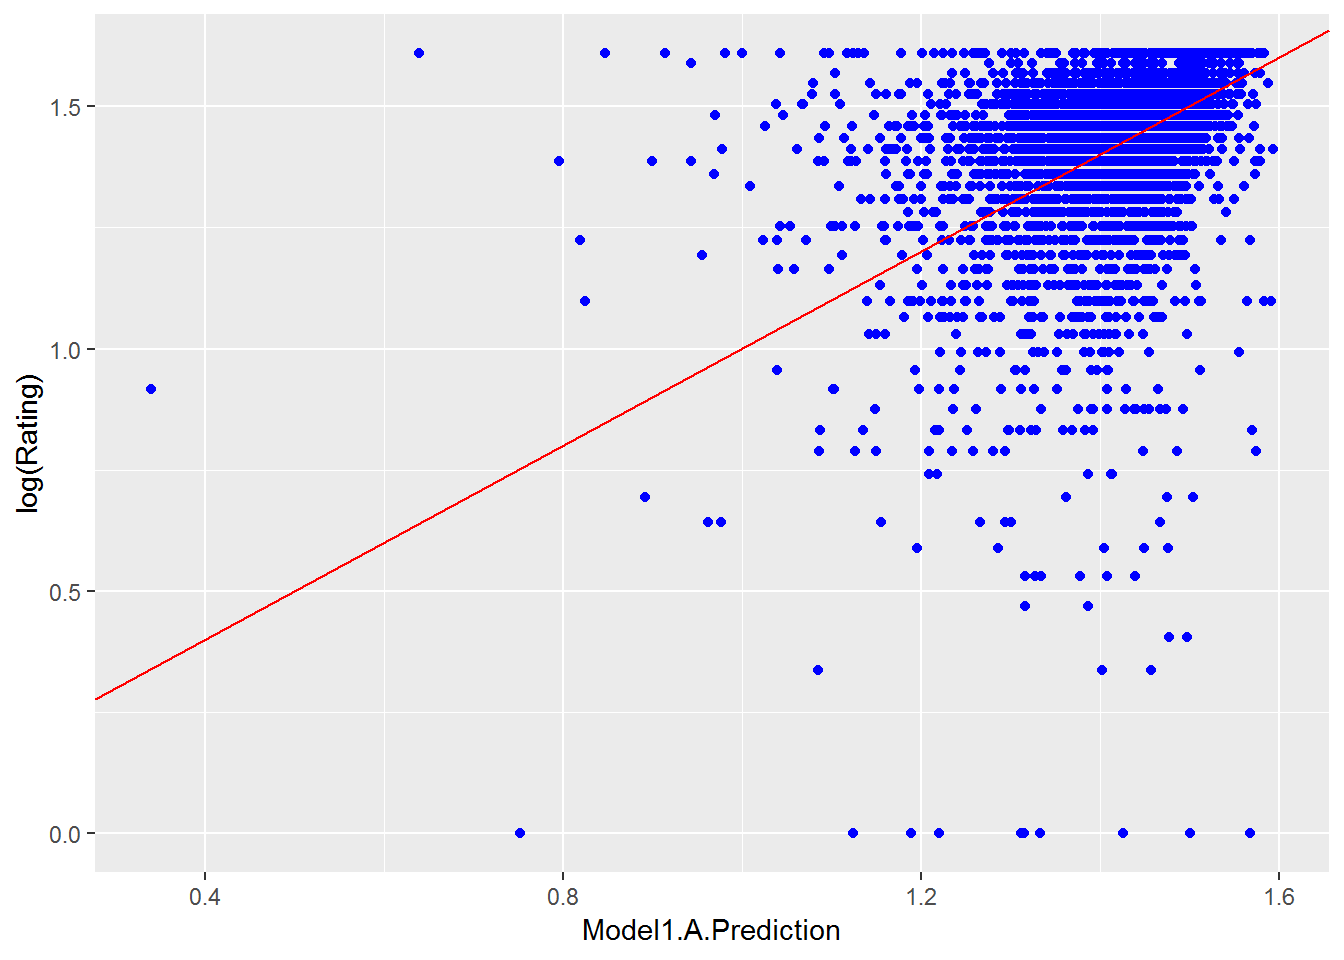
\includegraphics{Project_2_Work_files/figure-latex/unnamed-chunk-26-1.pdf}

\begin{Shaded}
\begin{Highlighting}[]
\KeywordTok{ggplot}\NormalTok{(Test) +}\StringTok{ }\KeywordTok{geom_point}\NormalTok{(}\KeywordTok{aes}\NormalTok{(}\DataTypeTok{x=}\NormalTok{Model1.A.Prediction.Test,}\DataTypeTok{y=}\KeywordTok{log}\NormalTok{(Rating)),}\DataTypeTok{color =} \StringTok{"green"}\NormalTok{) +}
\StringTok{  }\KeywordTok{geom_abline}\NormalTok{(}\DataTypeTok{intercept =} \DecValTok{0}\NormalTok{, }\DataTypeTok{color =} \StringTok{"red"}\NormalTok{)}
\end{Highlighting}
\end{Shaded}

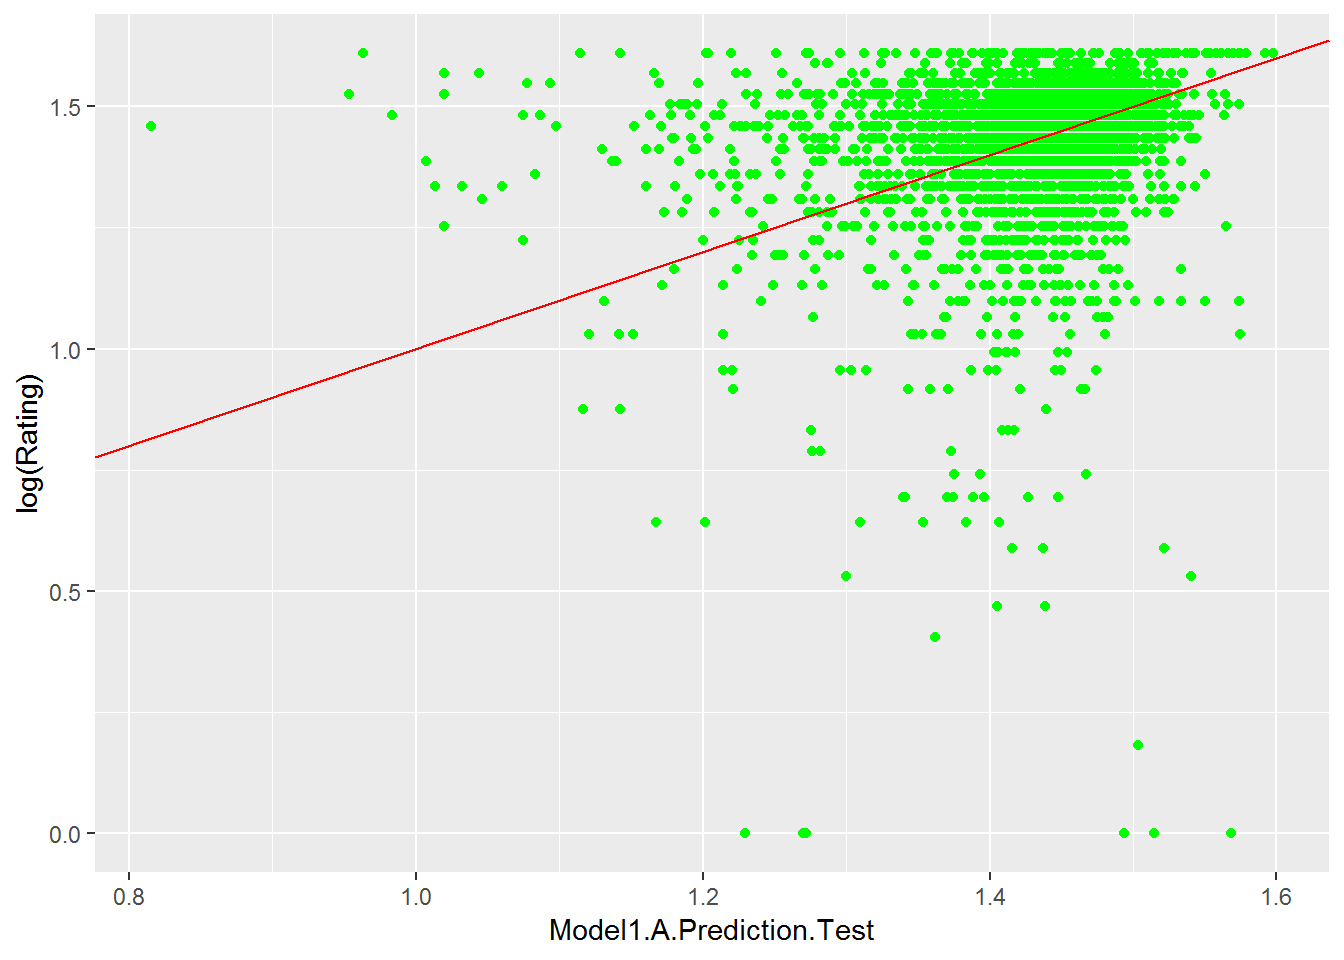
\includegraphics{Project_2_Work_files/figure-latex/unnamed-chunk-26-2.pdf}

\begin{Shaded}
\begin{Highlighting}[]
\KeywordTok{ggplot}\NormalTok{(Train) +}\StringTok{ }\KeywordTok{geom_point}\NormalTok{(}\KeywordTok{aes}\NormalTok{(}\DataTypeTok{x=}\NormalTok{Model2.A.Prediction,}\DataTypeTok{y=}\KeywordTok{log}\NormalTok{(Rating)),}\DataTypeTok{color =} \StringTok{"blue"}\NormalTok{) +}
\StringTok{  }\KeywordTok{geom_abline}\NormalTok{(}\DataTypeTok{intercept =} \DecValTok{0}\NormalTok{, }\DataTypeTok{color =} \StringTok{"red"}\NormalTok{)}
\end{Highlighting}
\end{Shaded}

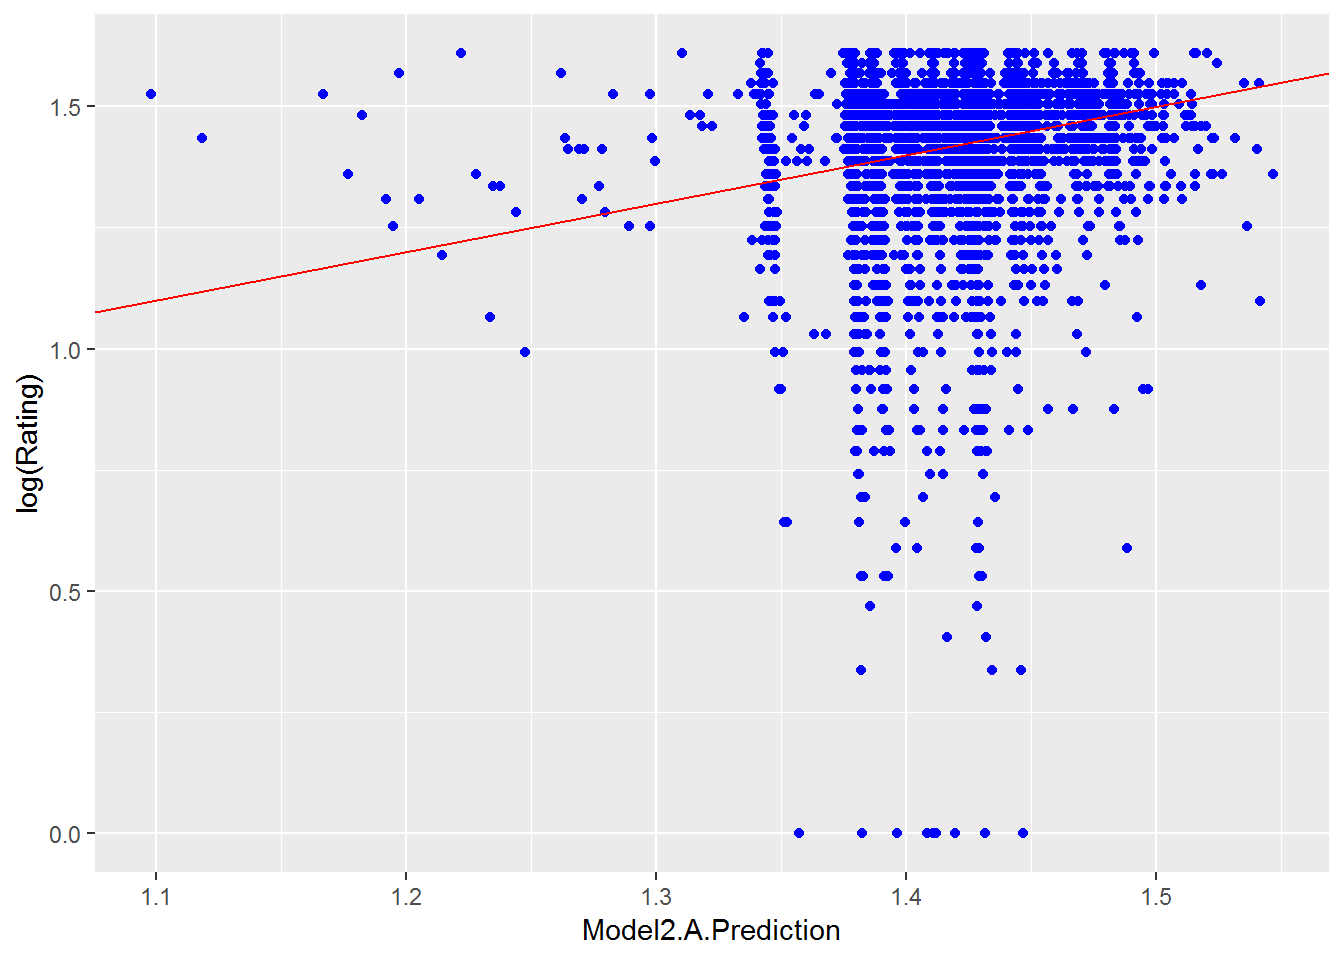
\includegraphics{Project_2_Work_files/figure-latex/unnamed-chunk-26-3.pdf}

\begin{Shaded}
\begin{Highlighting}[]
\KeywordTok{ggplot}\NormalTok{(Test) +}\StringTok{ }\KeywordTok{geom_point}\NormalTok{(}\KeywordTok{aes}\NormalTok{(}\DataTypeTok{x=}\NormalTok{Model2.A.Prediction.Test,}\DataTypeTok{y=}\KeywordTok{log}\NormalTok{(Rating)),}\DataTypeTok{color =} \StringTok{"green"}\NormalTok{) +}
\StringTok{  }\KeywordTok{geom_abline}\NormalTok{(}\DataTypeTok{intercept =} \DecValTok{0}\NormalTok{, }\DataTypeTok{color =} \StringTok{"red"}\NormalTok{)}
\end{Highlighting}
\end{Shaded}

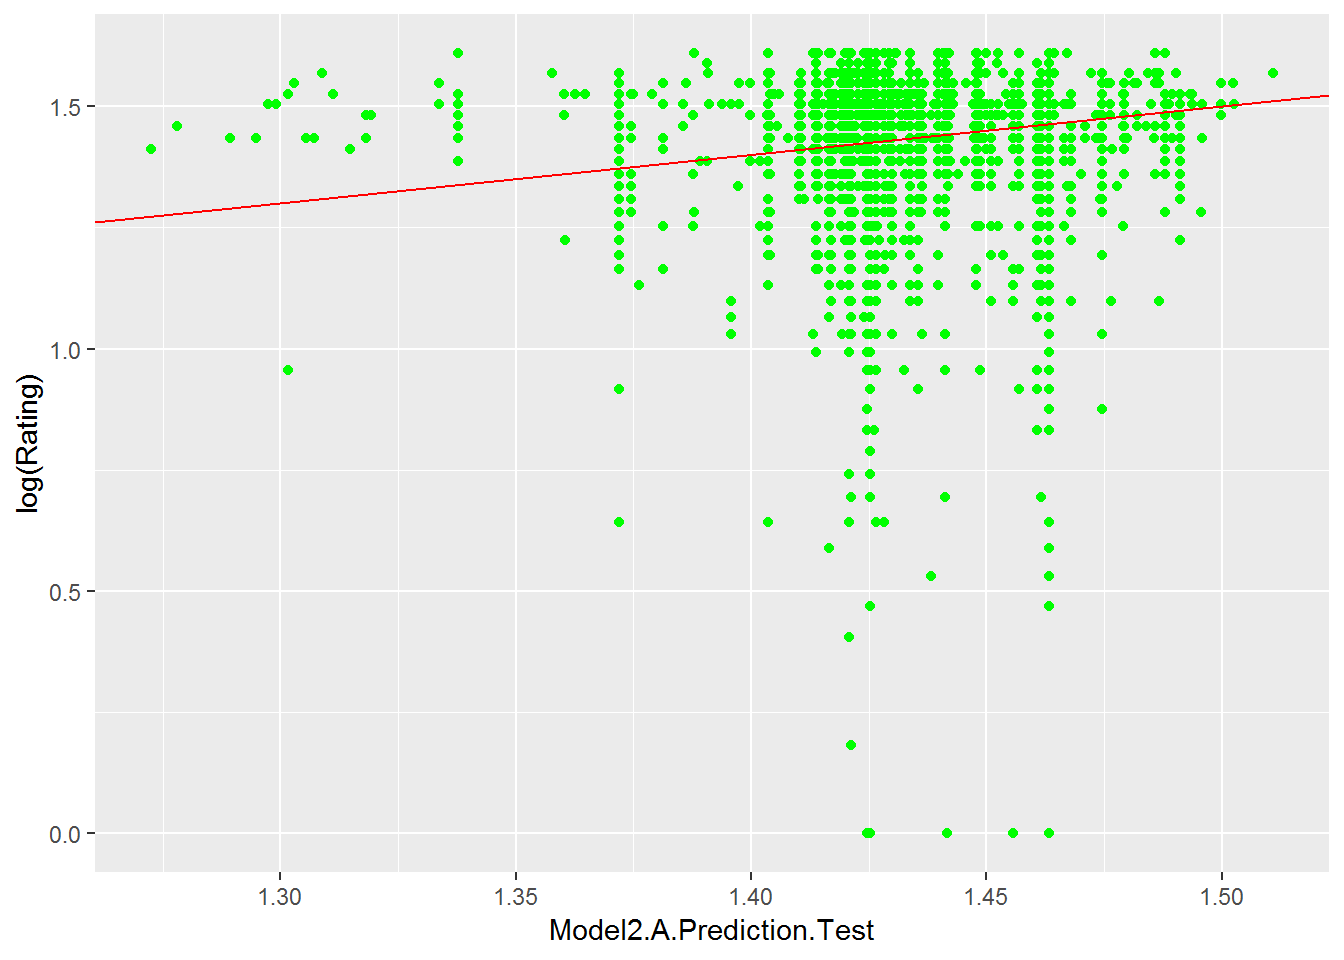
\includegraphics{Project_2_Work_files/figure-latex/unnamed-chunk-26-4.pdf}

\begin{Shaded}
\begin{Highlighting}[]
\KeywordTok{rm}\NormalTok{(Test)}
\end{Highlighting}
\end{Shaded}

These plots are the results of the models and their predictions. Blue
models are for training, green models are for testing. Model 1A is the
unconditional model. Model 2A is the conditional model.

\section{Discussion and Conclusions}\label{discussion-and-conclusions}

Overall, our models were not able to generate very accurate cases. In
both conditions, the models tended to overestimate the user rating
scores, especially for those who earned very low rating scores. While we
would like to believe this is due to the model's inherent optimism, we
feel that this is due to the majority of the user rating scores being
higher values, resulting in a predictive model which tends to moreso
pick higher ratings as its predictions. Also, it should be noted that
having the number of installations and the number of reviews greatly
aided in the predictive power of the model. This indicates that there is
a real correlation, however difficult to discern, between user-related
info and the user rating score. The models are not at all decent at what
they do; meaning that future work should strive to collect more data
from different variable sources to try and more accurately determine a
user rating score in advance. This would in turn force us to understand
what makes a good app and what people want in their apps. Provisionally
from this study, we can discern that, on average, a free, highly
downloaded, highly reviewed, rated E for Everyone app would most likely
lead to a high user rating score. Our research is important because it
shows that there is something to being able to predict a user rating
score. This is because the models, though sad as they might be, are not
completely incapable, suggesting some form of correlation somewhere.
Being able to predict a user rating score of an app before it launches
could be very helpful to businesses and corporations in deciding which
apps they will support, and which they will cast off to the side in
favor an app with a better predicted outcome on the market.


\end{document}
